%
%===================================================================================================
%
\documentclass[11pt,aspectratio=169,professionalfonts]{beamer}
%
%===================================================================================================
%
%
%===================================================================================================
%
% Main Modular Preamble Loader
%
%===================================================================================================

%
%===================================================================================================
%
% Packages
%
%===================================================================================================

\usepackage[absolute,overlay]{textpos}

\usepackage[utf8]{inputenc}
\usepackage[T1]{fontenc}

\usepackage{amsmath}
\usepackage{amsfonts}
\usepackage{amssymb}
% the following order matter!!!
\usepackage{lmodern}
\usepackage{bm}

\usepackage{array}
\usepackage{booktabs}
\usepackage{colortbl}
\usepackage{multirow}

\usepackage{graphicx}
\usepackage{tikz}
\usepackage{pgfplots}

\usepackage{framed}
\usepackage{empheq}

\usepackage{xcolor}
\usepackage{soul}

\usepackage{hyperref}
\usepackage{pgfpages}

%\usepackage{minted}

\usepackage[most]{tcolorbox}
\tcbuselibrary{listings}

\pgfplotsset{compat=1.14}
%
%===================================================================================================
%
% TikZ Libraries
%
%===================================================================================================

\usetikzlibrary{
    arrows.meta,
    positioning,
    fit,
    calc,
    shapes.geometric,
    backgrounds,
    matrix
}

% ── Reusable TikZ styles ─────────────────────────────────────
\tikzset{
  block/.style   = {draw, rounded corners, minimum width=2.0cm,
                    minimum height=0.60cm, align=center, font=\small},
  sblock/.style  = {draw, rounded corners, minimum width=1.4cm,
                    minimum height=0.55cm, align=center, font=\small},
  token/.style   = {draw, rounded corners, minimum width=1.1cm,
                    minimum height=0.55cm, font=\small},
  arr/.style     = {->, thick, boIndigo},
  arrg/.style    = {->, gray!60, line width=0.7pt}
}

%
%===================================================================================================
%
% Custom Colors
%
%===================================================================================================

% General accents
\definecolor{accent}{RGB}{200,60,50}
\definecolor{Accent}{RGB}{240,170,0}
\definecolor{accentblue}{HTML}{457B9D}
\definecolor{accentred}{HTML}{E63946}

% Course colors
\definecolor{CourseBlue}{RGB}{47,53,163}
\definecolor{unibo}{RGB}{0,68,136}
\definecolor{uniboblue}{RGB}{0,54,132}
\definecolor{uniblue}{RGB}{0,76,147}
\definecolor{unired}{RGB}{155,0,20}
\definecolor{codebg}{RGB}{248,248,248}
\definecolor{lightblue}{RGB}{220,235,250}

% Code colors
\definecolor{codebg}{rgb}{0.97,0.97,0.97}
\definecolor{codeborder}{rgb}{0.8,0.8,0.8}

% Neural-network / layer colors
\definecolor{w1col}{RGB}{255,180,0}
\definecolor{w2col}{RGB}{180,90,30}
\definecolor{b1col}{RGB}{0,255,0}
\definecolor{layer1violet}{HTML}{800080}
\definecolor{layer2red}{HTML}{FF0000}
\definecolor{updategreen}{HTML}{228B22}

% Financial colors
\definecolor{finblue}{RGB}{0,51,102}
\definecolor{fingray}{RGB}{100,100,100}
\definecolor{fingreen}{RGB}{0,100,0}
\definecolor{finred}{RGB}{178,34,34}

% Semantic colors
\definecolor{darkgreen}{RGB}{0,120,60}
\definecolor{DeepRed}{RGB}{180,45,45}
\definecolor{Forest}{RGB}{34,120,70}

% Light background colors
\definecolor{lightblue}{RGB}{210,230,250}
\definecolor{lightgreen}{RGB}{210,245,210}
\definecolor{lightorange}{RGB}{255,235,205}
\definecolor{lightred}{RGB}{255,220,220}
\definecolor{lightyellow}{RGB}{255,255,210}

% Soft background colors
\definecolor{SoftBlue}{RGB}{225,235,255}
\definecolor{SoftGray}{RGB}{245,245,245}
\definecolor{SoftGreen}{RGB}{228,243,232}
\definecolor{SoftOrange}{RGB}{255,244,224}

% Modern palette
\definecolor{navy}{RGB}{15,27,61}
\definecolor{deepblue}{RGB}{22,38,83}
\definecolor{midblue}{RGB}{30,58,110}
\definecolor{teal}{RGB}{13,148,136}
\definecolor{lightgray}{RGB}{148,163,184}
\definecolor{ice}{RGB}{202,220,252}
\definecolor{gold}{RGB}{245,158,11}
\definecolor{coral}{RGB}{249,115,22}
\definecolor{darktext}{RGB}{30,41,59}
\definecolor{offwhite}{RGB}{240,244,250}
\definecolor{boIndigo}{RGB}{55,0,153}

\definecolor{NavyBlue}{RGB}{20,40,100}
\definecolor{SteelBlue}{RGB}{70,130,180}
\definecolor{LightGray}{RGB}{245,245,250}
\definecolor{AccentGold}{RGB}{210,160,30}

\definecolor{futC} {gray}{0.60}
\definecolor{actC} {RGB}{15, 82, 186}
\definecolor{doneC}{RGB}{25, 25,  25}

\definecolor{GateOrange}{RGB}{230,120,0}
\definecolor{GatePurple}{RGB}{110,0,150}
\definecolor{CellGold}{RGB}{160,120,0}

% Alias
\colorlet{bolight}{boIndigo!10}
\colorlet{bodark}{boIndigo!85!black}
\colorlet{actFill}{actC!10}   % light-blue cell background when active


%
%===================================================================================================
%
% Beamer Theme and Style
%
%===================================================================================================

\usetheme{Madrid}
\usecolortheme{default}

%
%===================================================================================================
%
% Beamer Color Customization
%
%===================================================================================================

\setbeamercolor{title}{fg=white,bg=CourseBlue}
\setbeamercolor{frametitle}{fg=white,bg=CourseBlue}
\setbeamercolor{structure}{fg=CourseBlue}

\setbeamercolor{block title}{fg=white,bg=CourseBlue}
\setbeamercolor{block body}{fg=black,bg=SoftGray}

\setbeamercolor{item projected}{fg=white,bg=CourseBlue}

\setbeamercolor{section in head/foot}{fg=white,bg=CourseBlue}
\setbeamercolor{subsection in head/foot}{fg=white,bg=CourseBlue!80!black}
\setbeamercolor{author in head/foot}{fg=white,bg=CourseBlue!90!black}
\setbeamercolor{title in head/foot}{fg=white,bg=CourseBlue!70!black}
\setbeamercolor{date in head/foot}{fg=white,bg=CourseBlue!90!black}

%
%===================================================================================================
%
% Navigation Symbols and Itemize Style
%
%===================================================================================================

\setbeamertemplate{navigation symbols}{}

\setbeamertemplate{itemize item}{\color{CourseBlue}$\blacktriangleright$}
\setbeamertemplate{itemize subitem}{\color{CourseBlue}$\bullet$}
%
%===================================================================================================
%
% Mathematical Macros
%
%===================================================================================================

\newcommand{\vect}[1]{\bm{#1}}
\newcommand{\R}{\mathbb{R}}

\newcommand{\bx}{\bm{x}}
\newcommand{\bh}{\bm{h}}
\newcommand{\bw}{\bm{w}}
\newcommand{\bW}{\bm{W}}
\newcommand{\bb}{\bm{b}}
\newcommand{\diag}{\operatorname{diag}}

\newcommand{\vw}{\mathbf{w}}
\newcommand{\vwt}{\tilde{\mathbf{w}}}
%
%===================================================================================================
%
% Text and Highlighting Macros
%
%===================================================================================================

\newcommand{\soft}[1]{\textcolor{CourseBlue}{\textbf{#1}}}

\newcommand{\highlight}[1]{%
    \colorbox{yellow!25}{$\displaystyle #1$}
}

%
%===================================================================================================
%
% Beamer-Compatible Highlight Fix for the soul Package
%
%===================================================================================================

\makeatletter
\let\HL\hl
\renewcommand\hl{%
  \let\set@color\beamerorig@set@color
  \let\reset@color\beamerorig@reset@color
  \HL}
\makeatother

%
%===================================================================================================
%
% Custom Intuition Box
%
%===================================================================================================

\newcommand{\intuition}[1]{%
  \vspace{4pt}
  \begin{tikzpicture}
    \node[
        fill=offwhite,
        rounded corners=4pt,
        inner sep=6pt,
        text width=0.92\textwidth
    ] {%
      \textcolor{teal}{\textbf{Intuition:}} 
      \textcolor{darktext}{\small #1}
    };
  \end{tikzpicture}
}


\newcommand{\dmodel}{d_{\mathrm{model}}}
\newcommand{\dff}{d_{\mathrm{ff}}}
\newcommand{\dk}{d_k}
\newcommand{\dv}{d_v}

% ─────────────────────────────────────────────────────────────────────
%  \drawcell{cx}{cy}{border-color}{fill-color}
%  Draws the RNN cell rectangle + 3 neuron circles at (cx, cy).
% ─────────────────────────────────────────────────────────────────────
\newcommand{\drawcell}[4]{%
  \fill[#4, rounded corners=3pt]
    ({#1-0.68},{#2-1.10}) rectangle ({#1+0.68},{#2+1.10});
  \draw[color=#3, line width=1.5pt, rounded corners=3pt]
    ({#1-0.68},{#2-1.10}) rectangle ({#1+0.68},{#2+1.10});
  \draw[color=#3, line width=0.9pt] (#1,{#2+0.55}) circle(0.21);
  \draw[color=#3, line width=0.9pt] (#1, #2)        circle(0.21);
  \draw[color=#3, line width=0.9pt] (#1,{#2-0.55}) circle(0.21);
}
% Bold vectors shortcut (match existing notation)
\newcommand{\vct}[1]{\bm{#1}}

%
%===================================================================================================
%
\title{Chapter 2 -- Neural Networks and Static Word Embeddings}
\subtitle{Advanced Machine Learning for Finance}
\author{Giovanni Della Lunga}
\institute{University of Bologna}
\date{April-May 2026}
%
%===================================================================================================
%
\AtBeginSection[]{
\begin{frame}
\vfill
\centering
\begin{beamercolorbox}[sep=10pt,center,shadow=true,rounded=true]{title}
\usebeamerfont{title}\insertsectionhead\par
\end{beamercolorbox}
\vfill
\end{frame}
}
%
%===================================================================================================
%
\begin{document}
%
%===================================================================================================
%
\begin{frame}
    \titlepage
\end{frame}
%__________________________________________________________________________
%
\section{Introduction}
%__________________________________________________________________________
%
\begin{frame}{Where We Are in the Course}
\begin{block}{The general path of the course}
We started from \textbf{classical text representations}. Today we move to the first major transition: from hand-crafted lexical representations to \textbf{learned representations} and  to the basic logic of \textbf{neural language modeling}.
\end{block}

\vspace{0.2cm}
\begin{center}
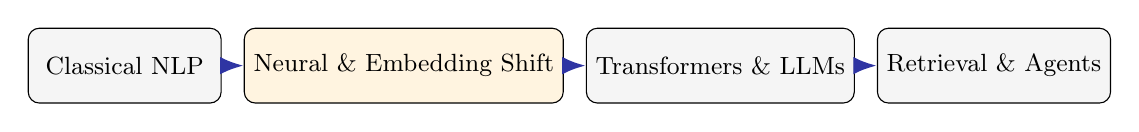
\begin{tikzpicture}[node distance=0.55cm and 0.28cm, every node/.style={font=\small}]
\node[draw, rounded corners, fill=SoftGray, minimum width=2.45cm, minimum height=0.95cm] (a) {Classical NLP};
\node[draw, rounded corners, fill=SoftOrange, right=of a, minimum width=2.75cm, minimum height=0.95cm] (b) {Neural \& Embedding Shift};
\node[draw, rounded corners, fill=SoftGray, right=of b, minimum width=2.45cm, minimum height=0.95cm] (c) {Transformers \& LLMs};
\node[draw, rounded corners, fill=SoftGray, right=of c, minimum width=2.45cm, minimum height=0.95cm] (d) {Retrieval \& Agents};
\draw[-{Latex[length=3mm]}, very thick, CourseBlue] (a) -- (b);
\draw[-{Latex[length=3mm]}, very thick, CourseBlue] (b) -- (c);
\draw[-{Latex[length=3mm]}, very thick, CourseBlue] (c) -- (d);
\end{tikzpicture}
\end{center}

\vspace{0.1cm}
\begin{itemize}
    \item Lesson 1 showed how text becomes data through sparse representations.
    \item Lesson 2 asks why sparse representations are not enough and how neural models begin to learn meaning.
\end{itemize}
\end{frame}
%
%..................................................................
%
\begin{frame}{Why This Lesson Matters}
\begin{columns}[T]
\begin{column}{0.49\textwidth}
\begin{block}{A conceptual reason}
Without a minimum understanding of neural networks, embeddings and LLMs easily look like magic. We need a compact but serious foundation.
\end{block}
\end{column}
\begin{column}{0.49\textwidth}
\begin{block}{A practical reason}
Many modern NLP systems are built on top of learned vector representations. Retrieval, ranking, semantic search, and generation all depend on this shift.
\end{block}
\end{column}
\end{columns}

\vspace{0.2cm}
\begin{alertblock}{Guiding question}
How do we move from \emph{counting words} to \emph{learning representations} that encode similarity, context, and structure?
\end{alertblock}
\end{frame}
%
%..................................................................
%
\begin{frame}{Where We Left Off}
In the previous lesson, text was represented mainly through:
\begin{itemize}
    \item sparse lexical indicators,
    \item term frequencies,
    \item inverse document frequencies,
    \item geometric similarity in high-dimensional spaces.
\end{itemize}

\vspace{0.2cm}
\begin{block}{What was missing?}
These representations are useful, interpretable, and computationally efficient, but they do not \textbf{learn} features. The model depends heavily on the representation we engineer by hand.
\end{block}

\vspace{0.1cm}
\begin{alertblock}{New idea}
What if the system itself could \textbf{learn} a useful representation while learning the task?
\end{alertblock}
\end{frame}
%
%..................................................................
%
\begin{frame}{Learning Objectives of Today's Lesson}
By the end of the lesson, students should be able to:
\begin{itemize}
    \item explain the difference between a perceptron, logistic regression, and a differentiable neuron;
    \item understand why gradient-based learning is a turning point for modern NLP;
    \item describe the intuition of distributional semantics and dense word vectors;
    \item explain the main logic of Word2Vec and the difference between CBOW and Skip-Gram;
    \item understand the role of co-occurrence in GloVe;
    \item identify the strengths and limitations of \textbf{static} embeddings.
\end{itemize}
\end{frame}
%
%..................................................................
%
\begin{frame}{Roadmap of the Lesson}
\tableofcontents
\end{frame}
%__________________________________________________________________________
%
\section{A Short Introduction to Deep Learning}
%__________________________________________________________________________
%
\begin{frame}{The Elementary Block: Three Instantiations}

The same functional form
\[
  \hat{y} = f(\mathbf{w}^{\top}\mathbf{x} + b)
\]
gives rise to three qualitatively different models depending on the choice of $f$.

\medskip
\begin{center}
\begin{tabular}{lll}
\hline
\textbf{Choice of $f$} & \textbf{Output} & \textbf{Task} \\
\hline\\
Identity $f(z)=z$ & real number & regression \\
Sign $f(z)=\operatorname{sgn}(z)$ & $\{-1,+1\}$ & hard classification \\
Sigmoid $f(z)=\sigma(z)$ & $(0,1)$ & probabilistic classification \\
\hline
\end{tabular}
\end{center}

\begin{block}{Reading direction}
Each choice removes one assumption of the previous one.
The three examples that follow build the conceptual path toward neural networks.
\end{block}

\end{frame}
%
%..................................................................
%
\begin{frame}{Instantiation 1 — Linear Regression ($f = \mathrm{Id}$)}

With $f(z) = z$ the block becomes
\[
  \hat{y} = \mathbf{w}^{\top}\mathbf{x} + b.
\]

\begin{columns}[T]
\begin{column}{0.48\textwidth}
\textbf{Setting.}
\begin{itemize}
  \item Input: a single feature $x$ (e.g.\ log-market-cap).
  \item Output: a continuous target $y$ (e.g.\ annual return).
  \item Loss: mean squared error
  \[
    \mathcal{L}(w,b) = \frac{1}{m}\sum_{i=1}^{m}(y_i - \hat{y}_i)^2.
  \]
  \item Update: gradient descent on $\mathcal{L}$.
\end{itemize}
\end{column}
\begin{column}{0.48\textwidth}
\vspace{0.5cm}
\begin{tikzpicture}[scale=0.85]
  \begin{axis}[
      width=9cm, height=7cm,
      xlabel={$x$}, ylabel={$\hat y$},
      xtick=\empty, ytick=\empty,
      axis lines=left,
      scatter/classes={a={mark=o,draw=blue!60,fill=blue!20,
                           mark size=1.8pt}},
  ]
  % scatter points
  \addplot[scatter,only marks,scatter src=explicit symbolic]
    coordinates {
      (0.5,1.2)[a] (1.0,1.8)[a] (1.5,2.6)[a]
      (2.0,3.1)[a] (2.5,3.9)[a] (3.0,4.4)[a]
      (0.8,1.5)[a] (1.8,2.9)[a] (2.8,4.1)[a]
      (1.2,2.0)[a] (2.2,3.4)[a]
    };
  % regression line
  \addplot[thick, red!70!black, domain=0.3:3.2]
    {1.4*x + 0.5};
  \node[red!70!black] at (axis cs:2.6,4.6) {$\hat y = wx+b$};
  \end{axis}
\end{tikzpicture}
\end{column}
\end{columns}

%\medskip
%\begin{alertblock}{Key point}
%The output is unbounded and continuous.
%No non-linearity means the model can only fit an affine relationship in the input space.
%The weight $w$ is interpretable directly as a marginal effect.
%\end{alertblock}

\end{frame}
%
%..................................................................
%
\begin{frame}{Instantiation 2 — Hard Classifier ($f = \operatorname{sgn}$)}

With $f(z) = \operatorname{sgn}(z)$ the block becomes
\[
  \hat{y} = \operatorname{sgn}(\mathbf{w}^{\top}\mathbf{x} + b)
  \in \{-1, +1\}.
\]

\begin{columns}[T]
\begin{column}{0.48\textwidth}
\textbf{Setting.}
\begin{itemize}
  \item Two linearly separable clusters in $\mathbb{R}^2$.
  \item The hyperplane $\mathbf{w}^{\top}\mathbf{x}+b=0$ is the decision boundary.
  \item Points on opposite sides receive opposite labels.
  \item Update rule: correct only on mistakes
        $\mathbf{w} \leftarrow \mathbf{w} + \eta\,y_i\,\mathbf{x}_i$.
\end{itemize}

%\medskip
%\begin{block}{Limitation}
%$\operatorname{sgn}$ is \textbf{not differentiable} at $0$
%and flat everywhere else.\\
%$\Rightarrow$ gradient descent has \emph{no signal} to follow.
%\end{block}

\end{column}
\begin{column}{0.48\textwidth}
\vspace{0.5cm}
\begin{tikzpicture}[scale=0.85]
  \begin{axis}[
      width=9cm, height=7cm,
      xlabel={$x_1$}, ylabel={$x_2$},
      xtick=\empty, ytick=\empty,
      axis lines=left,
      xmin=0, xmax=5, ymin=0, ymax=5,
  ]
  % class +1: top-left cluster (red circles)
  \addplot[only marks, mark=o,
           mark options={draw=red!80!black, fill=red!30},
           mark size=2pt]
    coordinates {(1.0,3.5)(1.2,4.2)(0.8,2.8)(1.5,4.0)
                 (0.6,3.2)(1.8,4.5)(1.0,2.5)};
  % class -1: bottom-right cluster (blue squares)
  \addplot[only marks, mark=square,
           mark options={draw=blue!80!black, fill=blue!20},
           mark size=2pt]
    coordinates {(3.5,1.2)(4.0,1.8)(3.0,0.8)(4.2,1.4)
                 (3.8,0.6)(2.8,1.6)(4.5,2.0)};
  % decision boundary: x2 = x1 - 0.5
  % separates top-left (+1) from bottom-right (-1)
  \addplot[thick, darkgray, dashed, domain=0.5:5.0]
    {x - 0.5};
  \node[darkgray, font=\scriptsize, rotate=45]
        at (axis cs:3.6,3.6)
        {$\mathbf{w}^\top\mathbf{x}+b=0$};
  \node[red!80!black, font=\small] at (axis cs:0.8,1.2)
        {$\hat y = +1$};
  \node[blue!80!black, font=\small] at (axis cs:4.2,2.8)
        {$\hat y = -1$};
  \end{axis}
\end{tikzpicture}
\end{column}
\end{columns}

\end{frame}
%
%..................................................................
%
\begin{frame}{Instantiation 3 — Probabilistic Classifier ($f = \sigma$)}

Replacing $\operatorname{sgn}$ with the sigmoid
$  \sigma(z) = 1/(1+e^{-z})$ gives a \textbf{smooth}, differentiable output in $(0,1)$:
\[
  P(y=1\mid\mathbf{x}) = \sigma(\mathbf{w}^{\top}\mathbf{x}+b).
\]

\begin{columns}[T]
\begin{column}{0.48\textwidth}
\vspace{0.5cm}
\begin{itemize}
  \item Same two clusters, but now the model
        outputs a \emph{probability}, not a hard label.
  \item Loss: binary cross-entropy
  \[
    \mathcal{L} = -\frac{1}{m}\sum_i
    \bigl[y_i \log a_i + (1{-}y_i)\log(1{-}a_i)\bigr].
  \]
  %\item $\sigma$ is differentiable: $\sigma'(z)=\sigma(z)(1-\sigma(z))$.\\
        %$\Rightarrow$ gradient descent \emph{has} a signal.
\end{itemize}

%\begin{alertblock}{Key gain}
%Differentiability of $f$ is what makes the chain rule work and
%allows us to stack layers — the foundation of deep learning.
%\end{alertblock}
\end{column}
\begin{column}{0.48\textwidth}
\vspace{0.5cm}
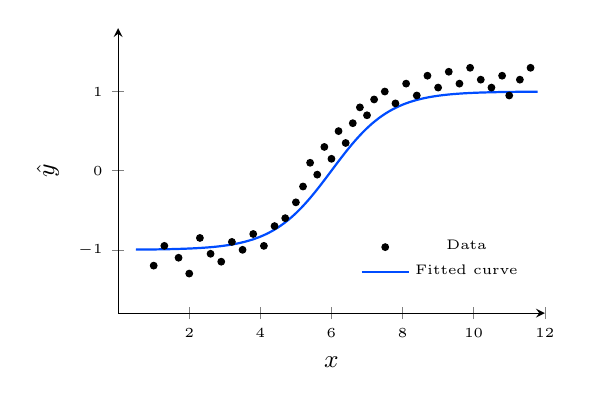
\begin{tikzpicture}
  \begin{axis}[
      width=7cm, height=5.2cm,
      xlabel={$x$},
      ylabel={$\hat{y}$},
      axis lines=left,
      xmin=0, xmax=12,
      ymin=-1.8, ymax=1.8,
      ytick={-1,0,1},
      xtick={2,4,6,8,10,12},
      tick label style={font=\tiny},
      label style={font=\small},
      legend style={
          at={(0.97,0.08)},
          anchor=south east,
          font=\tiny,
          draw=none,
          fill=none
      },
  ]

  %% noisy data points scattered around the sigmoid
  \addplot[
      only marks,
      mark=*,
      mark size=1.2pt,
      mark options={draw=black, fill=black},
  ] coordinates {
      (1.0,-1.20) (1.3,-0.95) (1.7,-1.10) (2.0,-1.30)
      (2.3,-0.85) (2.6,-1.05) (2.9,-1.15) (3.2,-0.90)
      (3.5,-1.00) (3.8,-0.80) (4.1,-0.95) (4.4,-0.70)
      (4.7,-0.60) (5.0,-0.40) (5.2,-0.20) (5.4, 0.10)
      (5.6,-0.05) (5.8, 0.30) (6.0, 0.15) (6.2, 0.50)
      (6.4, 0.35) (6.6, 0.60) (6.8, 0.80) (7.0, 0.70)
      (7.2, 0.90) (7.5, 1.00) (7.8, 0.85) (8.1, 1.10)
      (8.4, 0.95) (8.7, 1.20) (9.0, 1.05) (9.3, 1.25)
      (9.6, 1.10) (9.9, 1.30) (10.2,1.15) (10.5,1.05)
      (10.8,1.20) (11.0,0.95) (11.3,1.15) (11.6,1.30)
  };
  \addlegendentry{Data}

  %% fitted sigmoid: scaled to [-1, 1] range
  %% formula: 2*sigma(k*(x - x0)) - 1
  %% with k=1.2, x0=6
  \addplot[
      thick,
      color=blue!70!cyan,
      smooth,
      domain=0.5:11.8,
      samples=120,
  ] { 2/(1+exp(-1.2*(x-6))) - 1 };
  \addlegendentry{Fitted curve}

  \end{axis}
\end{tikzpicture}
\end{column}
\end{columns}

\end{frame}
%
%..................................................................
%
\begin{frame}{Why Neural Models Enter the Picture}
The simplest learning systems assign a label directly from the input:
\[
\hat{y} = f(\vect{w}^{\top}\vect{x} + b).
\]
If $f$ is a hard threshold or a linear function, the model draws a \textbf{fixed boundary} in the feature space we provide.

\vspace{0.2cm}
\begin{block}{The fundamental problem}
If the input features do not expose the right structure, no amount of optimization can compensate. The bottleneck is \textbf{representation}, not the optimizer.
\end{block}

\vspace{0.15cm}
\begin{alertblock}{Why this matters for NLP}
Text features engineered by hand --- counts, frequencies, indicators --- are static. Neural models are important because they can \textbf{learn} a better feature space jointly with the task, rather than being handed one.
\end{alertblock}
\end{frame}
%
%..................................................................
%
\begin{frame}{Three Related but Distinct Objects}

To understand how neural networks learn representations, we need to trace a short conceptual path through three objects that are closely related but serve distinct roles.

\vspace{0.25cm}

\centering
\small
\begin{tabular}{l l}
\toprule
\textbf{Object} & \textbf{Main idea} \\
\midrule
Perceptron          & Hard threshold decision rule with mistake-driven updates. \\[4pt]
Logistic regression & Probabilistic model for binary classification; smooth, differentiable loss. \\[4pt]
Sigmoid neuron      & Differentiable building block reusable inside neural networks. \\
\bottomrule
\end{tabular}

\raggedright
\vspace{0.2cm}
\begin{block}{Reading direction}
Each object removes one limitation of the previous one.
\end{block}
\end{frame}
%
%..................................................................
%
\begin{frame}{The Perceptron}
\begin{columns}[T]
\begin{column}{0.56\textwidth}
\begin{itemize}
    \item The perceptron is one of the earliest artificial neuron models.
    \item It performs a \textbf{hard} decision through a threshold rule:
    \[
    \hat{y} = \mathbb{I}(\vect{w}^{\top}\vect{x} + b \ge 0).
    \]
    \item It learns a \textbf{linear decision boundary}.
    \item It works on linearly separable problems, but fails on XOR-like patterns.
\end{itemize}
\end{column}
\begin{column}{0.40\textwidth}
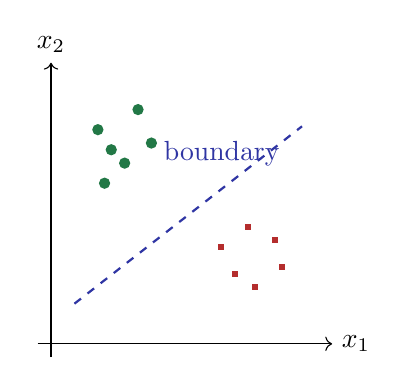
\begin{tikzpicture}[scale=0.85]
\draw[->] (-0.2,0) -- (4.2,0) node[right] {$x_1$};
\draw[->] (0,-0.2) -- (0,4.2) node[above] {$x_2$};
\foreach \x/\y in {0.7/3.2,1.1/2.7,1.3/3.5,0.9/2.9,1.5/3.0,0.8/2.4}
  \fill[Forest] (\x,\y) circle (2.4pt);
\foreach \x/\y in {2.7/1.0,3.3/1.5,3.0/0.8,2.9/1.7,3.4/1.1,2.5/1.4}
  \fill[DeepRed] (\x,\y) rectangle +(0.09,0.09);
\draw[thick,dashed,CourseBlue] (0.35,0.6) -- (3.75,3.25);
\node[CourseBlue] at (2.55,2.85) {boundary};
\end{tikzpicture}
\end{column}
\end{columns}
\end{frame}
%
%..................................................................
%
\begin{frame}{Perceptron Learning Rule}
Given a labeled example $(\vect{x}_i,y_i)$ with $y_i \in \{0,1\}$:
\[
\hat{y}_i = \mathbb{I}(\vect{w}^{\top}\vect{x}_i + b \ge 0)
\]
and update only on mistakes:
\[
\vect{w} \leftarrow \vect{w} + \eta(y_i - \hat{y}_i)\vect{x}_i,
\qquad
b \leftarrow b + \eta(y_i - \hat{y}_i).
\]

\vspace{0.2cm}
\begin{block}{Important clarification}
This is \textbf{not} gradient descent on cross-entropy. The activation is not differentiable, so the perceptron is historically important but not the right conceptual foundation for modern neural training.
\end{block}
\end{frame}
%
%..................................................................
%
\begin{frame}{What the Perceptron Is Not}
\begin{itemize}
    \item It is not a probabilistic model.
    \item It is not trained by maximizing likelihood.
    \item It is not trained by minimizing cross-entropy with gradient descent.
\end{itemize}

\vspace{0.25cm}
\begin{block}{Then why do we still teach it?}
\begin{itemize}
    \item It is conceptually simple.
    \item It makes the notion of linear separability explicit.
    \item It reveals a major limitation: a linear rule cannot solve every pattern.
    \item It motivates the move toward differentiable models.
\end{itemize}
\end{block}
\end{frame}
%
%..................................................................
%
\begin{frame}{Logistic Regression as a Probabilistic Model}
Instead of making a hard decision immediately, logistic regression models the conditional probability of class 1:
\[
P(y=1\mid \vect{x}) = \sigma(\vect{w}^{\top}\vect{x}+b),
\qquad
\sigma(t)=\frac{1}{1+e^{-t}}.
\]

\vspace{0.2cm}
\begin{itemize}
    \item The output lies in $(0,1)$.
    \item Labels are interpreted as Bernoulli random variables.
    \item The model remains linear in the input, but it is now \textbf{smooth and differentiable}.
\end{itemize}
\end{frame}
%
%..................................................................
%
\begin{frame}{Where the Loss Comes From}
If $a_i = \sigma(\vect{w}^{\top}\vect{x}_i+b)$, then:
\[
P(y_i\mid \vect{x}_i;\vect{w},b)=a_i^{y_i}(1-a_i)^{1-y_i}.
\]
Taking logs and summing over the sample leads to the log-likelihood:
\[
\log L(\vect{w},b)=\sum_{i=1}^{m}\left[y_i\log a_i + (1-y_i)\log(1-a_i)\right].
\]
Maximizing this quantity is equivalent to minimizing the binary cross-entropy:
\[
\mathcal{L}(\vect{w},b)= -\frac{1}{m}\sum_{i=1}^{m}\left[y_i\log a_i + (1-y_i)\log(1-a_i)\right].
\]
\end{frame}
%
%..................................................................
%
\begin{frame}{From Differentiable Activation to Differentiable Loss}
The loss for logistic regression is a composition of functions:
\[
\mathcal{L}(\vect{w},b)
= -\frac{1}{m}\sum_{i=1}^{m}\Bigl[y_i\log\underbrace{\sigma(\vect{w}^{\top}\vect{x}_i+b)}_{a_i}
  + (1-y_i)\log(1-\underbrace{\sigma(\vect{w}^{\top}\vect{x}_i+b)}_{a_i})\Bigr].
\]

\vspace{0.1cm}
Differentiating with respect to $w_j$ via the chain rule:
\[
\frac{\partial \mathcal{L}}{\partial w_j}
= \frac{\partial \mathcal{L}}{\partial a_i}\cdot
  \underbrace{\frac{\partial a_i}{\partial z_i}}_{\sigma'(z_i)}\cdot
  \frac{\partial z_i}{\partial w_j}
= \frac{1}{m}\sum_{i=1}^{m}(a_i - y_i)\,x_{ij}.
\]

\vspace{0.05cm}
\begin{block}{Why differentiability of $\sigma$ is essential}
The middle term $\sigma'(z) = \sigma(z)(1-\sigma(z))$ is what makes the chain rule close.
If the activation were a hard threshold (as in the perceptron), $\sigma' = 0$ almost everywhere and gradient descent would have no signal to follow.
\end{block}
\end{frame}
%
%..................................................................
%
\begin{frame}{From Differentiable Activation to Differentiable Loss}
\begin{alertblock}{Key message}
Choosing a \textbf{differentiable} activation function is not a cosmetic detail: it is what makes the loss itself differentiable with respect to the model parameters.
\end{alertblock}
\end{frame}
%
%..................................................................
%
\begin{frame}{Why Logistic Regression Fits the Neural View}
\begin{columns}[T]
\begin{column}{0.52\textwidth}
\begin{block}{Two crucial ingredients}
\begin{itemize}
    \item \textbf{Differentiability}: $\sigma(\cdot)$ is differentiable.
    \item \textbf{Smooth objective}: cross-entropy works naturally with gradients.
\end{itemize}
\end{block}

\vspace{0.15cm}
\begin{alertblock}{Bridge to deep learning}
Differentiable model + differentiable loss $\Rightarrow$ gradient-based training.
\end{alertblock}
\end{column}
\begin{column}{0.43\textwidth}
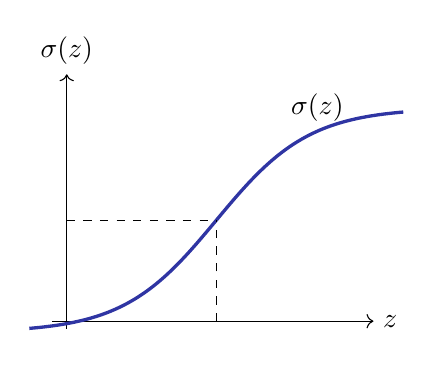
\begin{tikzpicture}[scale=0.95]
\draw[->] (-0.2,0) -- (4.1,0) node[right] {$z$};
\draw[->] (0,-0.1) -- (0,3.3) node[above] {$\sigma(z)$};
\draw[CourseBlue, very thick, domain=-4:4, smooth, samples=100] plot (\x/1.6+2,{3/(1+exp(-\x))-0.15});
\draw[dashed] (2,0) -- (2,1.35);
\draw[dashed] (0,1.35) -- (2,1.35);
\node at (3.35,2.85) {$\sigma(z)$};
\end{tikzpicture}
\end{column}
\end{columns}
\end{frame}
%
%..................................................................
%
\begin{frame}{Gradient Descent in Vector Form}
For logistic regression, the gradient takes a compact form:
\[
\nabla_{\vect{w}}\mathcal{L}=\frac{1}{m}X^{\top}(A-y),
\qquad
\frac{\partial \mathcal{L}}{\partial b}=\frac{1}{m}\mathbf{1}^{\top}(A-y).
\]

\vspace{0.2cm}
\begin{itemize}
    \item $A-y$ is the prediction error in probability space.
    \item Updating the parameters means moving them against the gradient:
    \[
    \vect{w} \leftarrow \vect{w} - \eta \nabla_{\vect{w}}\mathcal{L},
    \qquad
    b \leftarrow b - \eta \frac{\partial \mathcal{L}}{\partial b}.
    \]
    \item The same pattern will later reappear in backpropagation.
\end{itemize}
\end{frame}
%
%..................................................................
%
\begin{frame}{The Sigmoid Neuron}
\begin{columns}[T]
\begin{column}{0.57\textwidth}
A sigmoid neuron performs two operations:
\[
z = \vect{w}^{\top}\vect{x}+b,
\qquad
a = \sigma(z).
\]

\vspace{0.15cm}
\begin{itemize}
    \item a linear combination of the inputs,
    \item followed by a nonlinear activation.
\end{itemize}

\vspace{0.15cm}
\begin{block}{Why it matters}
This is the atomic operation that neural networks will repeat layer after layer.
\end{block}
\end{column}
\begin{column}{0.38\textwidth}
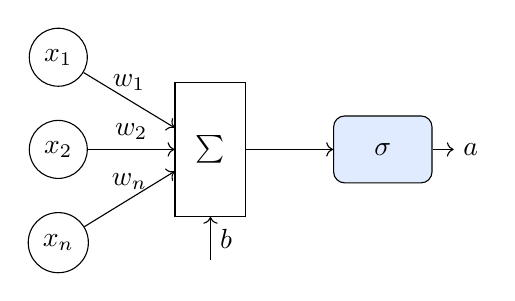
\begin{tikzpicture}[node distance=0.42cm]
\node[circle,draw] (x1) {$x_1$};
\node[circle,draw,below=of x1] (x2) {$x_2$};
\node[circle,draw,below=of x2] (x3) {$x_n$};
\node[draw,rectangle,minimum width=0.9cm,minimum height=1.7cm,right=1.1cm of x2] (sum) {$\sum$};
\node[draw,rounded corners,fill=SoftBlue,minimum width=1.25cm,minimum height=0.85cm,right=1.1cm of sum] (sig) {$\sigma$};
\draw[->] (x1) -- node[above] {$w_1$} (sum);
\draw[->] (x2) -- node[above] {$w_2$} (sum);
\draw[->] (x3) -- node[above] {$w_n$} (sum);
\draw[->] (sum) -- (sig);
\draw[->] (sig) -- ++(0.9,0) node[right] {$a$};
\draw[->] ($(sum.south)+(0,-0.55)$) -- node[right] {$b$} (sum.south);
\end{tikzpicture}
\end{column}
\end{columns}
\end{frame}
%
%..................................................................
%
\begin{frame}{A Limitation of Single-Neuron Models}
\begin{itemize}
    \item A logistic neuron can optimize its parameters very well.
    \item But no amount of optimization can make a single linear boundary solve a truly nonlinear pattern.
    \item The limitation is therefore not only optimization -- it is also \textbf{representation}.
\end{itemize}

\vspace{0.2cm}
\begin{alertblock}{Key idea}
If the original coordinates do not expose the right structure, we need a mechanism that learns a \textbf{new coordinate system}.
\end{alertblock}
\end{frame}
%
%..................................................................
%
\begin{frame}{The XOR Problem}

\begin{columns}[T]
\begin{column}{0.52\textwidth}

\includegraphics[scale=.5]{../05-pictures/chapter-02_pic_0.png}
\end{column}
\begin{column}{0.45\textwidth}
\textbf{Problem definition.}

\medskip
Class assignment depends on a \emph{nonlinear} rule:
\[
  y = 1 \;\;\text{iff}\;\; x_1 x_2 > 0
\]
i.e.\ points in \textbf{Quadrants I and III} belong to
\textcolor{accentred}{Class~1}, the rest to
\textcolor{accentblue}{Class~0}.

\bigskip
This is the classic \alert{XOR-like} pattern:
the label depends on the \emph{product} (interaction)
of the two features, not on each feature alone.
\end{column}
\end{columns}

\end{frame}
%
%..................................................................
%
\begin{frame}{Why a Single Neuron Fails}

\begin{columns}[T]
\begin{column}{0.52\textwidth}

\includegraphics[scale=.5]{../05-pictures/chapter-02_pic_1.png}
\end{column}
\begin{column}{0.45\textwidth}
No matter which line we try:
\[
  w_1 x_1 + w_2 x_2 + b = 0
\]
it \textbf{always} misclassifies a substantial fraction
of the data.

\bigskip
\textbf{The problem is not optimization.}

A logistic neuron can find the best possible line
--- but no line is good enough.

\bigskip
\alert{The problem is the \textbf{representation}:}
the raw features $(x_1, x_2)$ do not expose the
structure needed for a linear decision.
\end{column}
\end{columns}

\end{frame}
%
%..................................................................
%
\begin{frame}{The Core Idea: Learn a New Coordinate System}

\begin{block}{Key insight (Goodfellow et al., Ch.~6)}
Instead of classifying in the \emph{original} space, transform the
input into a \textbf{new space} where the problem \emph{becomes}
linearly separable.
\end{block}

\vspace{0.2cm}
Introduce a \alert{hidden layer} $\bh(\bx)$ with two neurons:
\[
  h_j(\bx) \;=\; \sigma\!\bigl(\bw_j^{\!\top}\bx + b_j\bigr),
  \qquad j = 1, 2
\]

Then classify in the \emph{transformed} space:
\[
  \bx \;\;\xrightarrow{\;\;\bh(\bx)\;\;}\;\;
  (h_1, h_2) \;\;\xrightarrow{\;\text{linear}\;\;}\;\; \hat{y}
\]

\vspace{0.2cm}
\textbf{The hidden layer does not add complexity for its own sake.}\\
It \emph{builds a coordinate system} in which a hyperplane suffices.

\end{frame}
%
%..................................................................
%
\begin{frame}{The Core Idea: Learn a New Coordinate System}
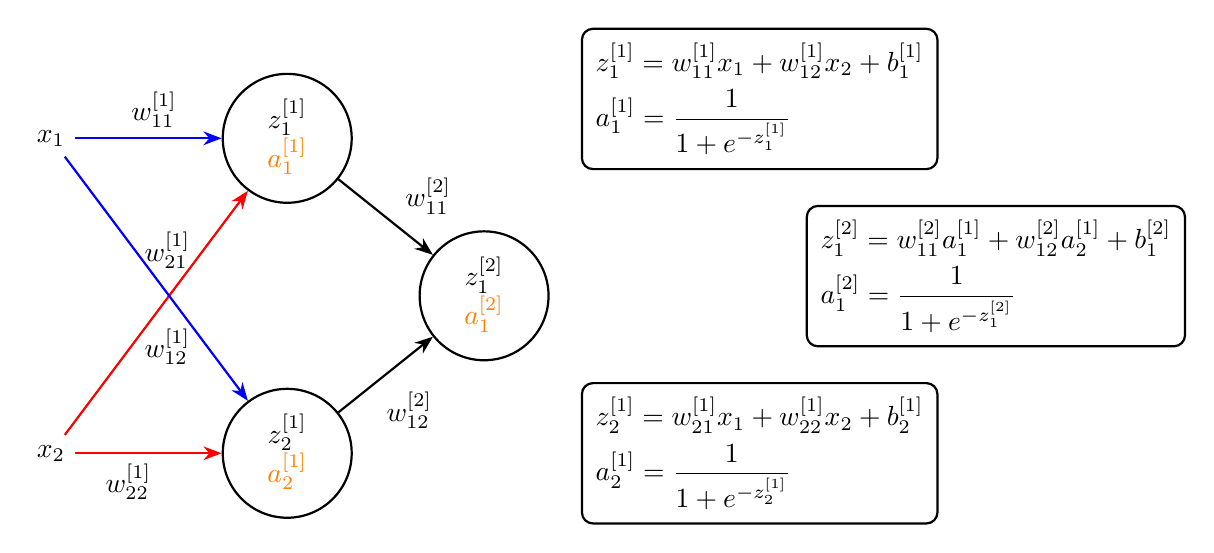
\begin{tikzpicture}[
    neuron/.style={circle, draw, minimum size=1em},
    input/.style={},
    ->, thick, >=Stealth
]

% --- INPUT NODES ---
\node[input] (x1) at (0,4) {$x_1$};
\node[input] (x2) at (0,0) {$x_2$};

% --- HIDDEN LAYER NEURONS ---
\node[neuron] (z1_1) at (3,4) {$\begin{array}{c} z_1^{[1]} \\ \textcolor{orange}{a_1^{[1]}} \end{array}$};
\node[neuron] (z2_1) at (3,0) {$\begin{array}{c} z_2^{[1]} \\ \textcolor{orange}{a_2^{[1]}} \end{array}$};

% --- OUTPUT NEURON ---
\node[neuron] (z1_2) at (5.5,2) {$\begin{array}{c} z_1^{[2]} \\ \textcolor{orange}{a_1^{[2]}}\end{array}$};
% centered between z1 and z2

% --- CONNECTIONS: INPUT TO HIDDEN ---
\draw[draw=blue] (x1) -- node[above, xshift=2pt] {$w_{11}^{[1]}$} (z1_1);
\draw[draw=red]  (x2) -- node[below, xshift=4pt, yshift=-2pt] {$w_{12}^{[1]}$} (z1_1);
\draw[draw=blue] (x1) -- node[above, xshift=4pt] {$w_{21}^{[1]}$} (z2_1);
\draw[draw=red]  (x2) -- node[below, pos=0.4, xshift=-2pt] {$w_{22}^{[1]}$} (z2_1);

% --- BIAS TO HIDDEN LAYER ---
%\node[input] (b1) at (2,3.2) {};
%\node[input] (b2) at (2,-1.2) {};
%\draw[->] (b1) -- (z1_1) node[midway, left, xshift=-2pt] {$b_1$};
%\draw[->] (b2) -- (z2_1) node[midway, left, xshift=-2pt] {$b_2$};

% --- CONNECTIONS: HIDDEN TO OUTPUT ---
\draw (z1_1) -- node[above right, pos=0.6] {$w_{11}^{[2]}$} (z1_2);
\draw (z2_1) -- node[below right, pos=0.4] {$w_{12}^{[2]}$} (z1_2);

% --- BIAS TO OUTPUT NODE ---
%\node[input] (b3) at (5,2.5) {};
%\draw[->] (b3) -- (z1_2) node[midway, left] {$b_3$};

% --- EQUATIONS FOR HIDDEN LAYER ---
\node[align=left, draw, rounded corners, inner sep=5pt] at (9,4.5) {
    $\displaystyle z_1^{[1]} = w_{11}^{[1]}x_1 + w_{12}^{[1]}x_2 + b_1^{[1]}$\\[0.3em]
    $\displaystyle a_1^{[1]} = \frac{1}{1 + e^{-z_1^{[1]}}}$
};

\node[align=left, draw, rounded corners, inner sep=5pt] at (9,0) {
    $\displaystyle z_2^{[1]} = w_{21}^{[1]}x_1 + w_{22}^{[1]}x_2 + b_2^{[1]}$\\[0.3em]
    $\displaystyle a_2^{[1]} = \frac{1}{1 + e^{-z_2^{[1]}}}$
};

% --- OUTPUT EQUATION ---
\node[align=left, draw, rounded corners, inner sep=5pt] at (12,2.25) {
    $\displaystyle z_1^{[2]} = w_{11}^{[2]}a_1^{[1]} + w_{12}^{[2]}a_2^{[1]} + b_1^{[2]}$\\[0.3em]
    $\displaystyle a_1^{[2]} = \frac{1}{1 + e^{-z_1^{[2]}}}$
};
\end{tikzpicture}
\end{frame}
%
%..................................................................
%
\begin{frame}{What Each Hidden Neuron Computes}

\begin{center}

\includegraphics[scale=.5]{../05-pictures/chapter-02_pic_2.png}
\end{center}

{\small
Each neuron partitions the original space with its own
\emph{linear boundary} and then ``squashes'' the result
through $\sigma$.
Individually, neither $h_1$ nor $h_2$ separates the classes
--- but \textbf{together} they create a representation where
a linear classifier succeeds.
}

\end{frame}
%
%..................................................................
%
\begin{frame}{Tracking Points: From $(x_1, x_2)$ to $(h_1, h_2)$}

\vspace{-4pt}
\begin{center}

\includegraphics[scale=.4]{../05-pictures/chapter-02_pic_3.png}
\end{center}

\vspace{-6pt}
{\footnotesize
\begin{tabular}{lccccl}
\toprule
 & $(x_1, x_2)$ & Quadrant & $h_1$ & $h_2$ & New coords \\
\midrule
$P_1$ & $(+0.79,\;+0.56)$ & I\;\textcolor{accentred}{(cls\,1)}
      & $0.59$ & $1.00$ & $(0.59,\; 1.00)$ \\
$P_2$ & $(-0.83,\;-0.59)$ & III\;\textcolor{accentred}{(cls\,1)}
      & $0.00$ & $0.27$ & $(0.00,\; 0.27)$ \\
$P_3$ & $(-1.17,\;+2.31)$ & II\;\textcolor{accentblue}{(cls\,0)}
      & $0.39$ & $1.00$ & $(0.39,\; 1.00)$ \\
$P_4$ & $(+1.46,\;-0.21)$ & IV\;\textcolor{accentblue}{(cls\,0)}
      & $0.47$ & $1.00$ & $(0.47,\; 1.00)$ \\
\bottomrule
\end{tabular}
\hfill
\parbox[b]{0.38\linewidth}{\raggedright
\textbf{Recipe:} read $h_1$ from the left panel, $h_2$ from the center.
The pair $(h_1, h_2)$ is the new address in the right panel.
}
}

\end{frame}
%
%..................................................................
%
\begin{frame}{The Transformed Space Is Linearly Separable}

\begin{columns}[T]
\begin{column}{0.52\textwidth}

\includegraphics[scale=.55]{../05-pictures/chapter-02_pic_4.png}
\end{column}
\begin{column}{0.45\textwidth}
After the hidden layer, each point $\bx$ is mapped
to coordinates $(h_1, h_2) \in (0,1)^2$.

\bigskip
In this new space the two classes occupy
\textbf{separable clusters}.

\bigskip
A single linear boundary
\[
  w_1' h_1 + w_2' h_2 + b' = 0
\]
now suffices (black line).

\bigskip
\alert{This is exactly what the output neuron does:}
it is a logistic regression in $\bh$-space.
\end{column}
\end{columns}

\end{frame}
%
%..................................................................
%
\begin{frame}{Side by Side: Original $\to$ Transformed}

\begin{center}

\includegraphics[scale=.45]{../05-pictures/chapter-02_pic_5.png}
\end{center}

\vspace{-4pt}
{\small
\textbf{Left:} no linear boundary works.
\hfill
\textbf{Right:} after $\bh(\bx)$, a straight line is all we need.

\smallskip
The hidden layer has \emph{learned} the feature interaction
that we would have had to engineer by hand (e.g.\ $x_1 x_2$).
}

\end{frame}
%
%..................................................................
%
\begin{frame}{The Decision Boundary Back in the Original Space}

\begin{columns}[T]
\begin{column}{0.52\textwidth}

\includegraphics[scale=.55]{../05-pictures/chapter-02_pic_6.png}
\end{column}
\begin{column}{0.45\textwidth}
When we map the linear boundary from $\bh$-space
\textbf{back} to $(x_1, x_2)$-space, it becomes a
\alert{nonlinear curve}.

\bigskip
The network has effectively learned:
\begin{enumerate}
\item A nonlinear feature map $\bh(\bx)$
\item A linear classifier in that space
\end{enumerate}

\bigskip
\textbf{Together}, these two steps produce a
complex decision boundary --- while each step
alone is simple.

\bigskip
This is the fundamental architecture of
\emph{every} feedforward neural network.
\end{column}
\end{columns}

\end{frame}
%
%..................................................................
%
\begin{frame}{From Direct Prediction to Representation Learning}
Instead of learning
\[
\vect{x} \longrightarrow y
\]
we can learn
\[
\vect{x} \longrightarrow h(\vect{x}) \longrightarrow y.
\]

\vspace{0.2cm}
\begin{block}{Interpretation}
The hidden layer does not add complexity for its own sake. It constructs a new feature space in which a simple linear classifier may become sufficient.
\end{block}

\vspace{0.15cm}
\begin{itemize}
    \item Classical machine learning often follows: \textit{feature engineering $\rightarrow$ model}.
    \item Neural networks aim at: \textit{model $\rightarrow$ features $\rightarrow$ prediction}.
\end{itemize}
\end{frame}
%
%..................................................................
%
\begin{frame}{What a Feedforward Neural Network Really Does}
A feedforward network repeatedly applies two steps:
\[
\text{linear map} \quad z = W x + b
\qquad \Longrightarrow \qquad
\text{nonlinear map} \quad a = \phi(z).
\]

\vspace{0.2cm}
\begin{center}
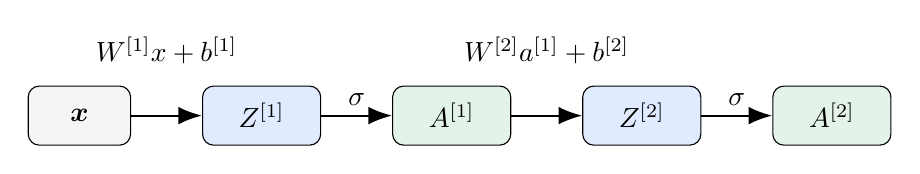
\begin{tikzpicture}[node distance=0.9cm and 0.9cm]
\node[draw,rounded corners,fill=SoftGray,minimum width=1.3cm,minimum height=0.75cm] (x) {$\vect{x}$};
\node[draw,rounded corners,fill=SoftBlue,right=of x,minimum width=1.5cm,minimum height=0.75cm] (z1) {$Z^{[1]}$};
\node[draw,rounded corners,fill=SoftGreen,right=of z1,minimum width=1.5cm,minimum height=0.75cm] (a1) {$A^{[1]}$};
\node[draw,rounded corners,fill=SoftBlue,right=of a1,minimum width=1.5cm,minimum height=0.75cm] (z2) {$Z^{[2]}$};
\node[draw,rounded corners,fill=SoftGreen,right=of z2,minimum width=1.5cm,minimum height=0.75cm] (a2) {$A^{[2]}$};
\draw[-{Latex[length=3mm]},thick] (x) -- node[above, yshift=15pt] {$W^{[1]}x+b^{[1]}$} (z1);
\draw[-{Latex[length=3mm]},thick] (z1) -- node[above] {$\sigma$} (a1);
\draw[-{Latex[length=3mm]},thick] (a1) -- node[above, yshift=15pt] {$W^{[2]}a^{[1]}+b^{[2]}$} (z2);
\draw[-{Latex[length=3mm]},thick] (z2) -- node[above] {$\sigma$} (a2);
\end{tikzpicture}
\end{center}

\vspace{0.15cm}
\begin{block}{Core idea}
A neural network is a \textbf{composition of functions}. Backpropagation is simply the differentiation of this composition.
\end{block}
\end{frame}
%
%..................................................................
%
\begin{frame}{Remind: Neural Networks Are Supervised Learners}
 
Everything we have built so far is an instance of \textbf{supervised learning}.
 
\bigskip
 
\begin{block}{What supervised learning requires}
\begin{itemize}
  \item A \textbf{labelled dataset} $\{(\bx^{(i)}, y^{(i)})\}_{i=1}^{m}$ — inputs paired with known targets.
  \item A \textbf{model} that maps inputs to predictions: $\hat{y} = f_\theta(\bx)$.
  \item A \textbf{loss function} $\mathcal{L}(\theta)$ that measures how far $\hat{y}$ is from $y$.
  \item An \textbf{optimiser} that adjusts $\theta$ to reduce $\mathcal{L}$.
\end{itemize}
\end{block}
 
\end{frame}
%
%..................................................................
%
\begin{frame}{The Optimization Problem and the Training Loop}
We have seen that a feedforward network computes
\[
\hat{y} = A^{[2]} = \sigma\!\bigl(W^{[2]}\,\sigma(W^{[1]}X + b^{[1]}) + b^{[2]}\bigr).
\]
The binary cross-entropy loss measures how far the predictions are from the labels:
\[
\mathcal{L}\!\bigl(W^{[1]}, b^{[1]}, W^{[2]}, b^{[2]}\bigr)
= -\frac{1}{m}\sum_{i=1}^{m}\Bigl[y_i\log A^{[2]}_i + (1-y_i)\log(1-A^{[2]}_i)\Bigr].
\]

\vspace{0.15cm}
\begin{block}{What we need}
To apply gradient descent we must compute
\[
\frac{\partial \mathcal{L}}{\partial W^{[1]}},\quad
\frac{\partial \mathcal{L}}{\partial b^{[1]}},\quad
\frac{\partial \mathcal{L}}{\partial W^{[2]}},\quad
\frac{\partial \mathcal{L}}{\partial b^{[2]}}.
\]
\end{block}
\end{frame}
%
%..................................................................
%
\begin{frame}{The Optimization Problem and the Training Loop}
 
The abstract supervised learning cycle instantiates, for our two-layer network, as follows.
 
\bigskip
 
\begin{columns}[T]
\small 
\begin{column}{0.52\textwidth}
\begin{block}{One training step}
\begin{enumerate}
  \item \textbf{Forward pass.} Given a batch $\{(\bx^{(i)}, y^{(i)})\}$, compute:
  \[
    A^{[1]} = \sigma(W^{[1]}X + b^{[1]}), \quad
    A^{[2]} = \sigma(W^{[2]}A^{[1]} + b^{[2]}).
  \]
  \item \textbf{Loss.} Compute the binary cross-entropy $\mathcal{L}(A^{[2]}, y)$.
  \item \textbf{Backward pass.} Apply backpropagation to obtain $\nabla_{W^{[\ell]}}\mathcal{L}$, $\nabla_{b^{[\ell]}}\mathcal{L}$.
  \item \textbf{Update.} $\theta \leftarrow \theta - \eta\,\nabla_\theta \mathcal{L}$.
\end{enumerate}
\end{block}
\end{column}
 
\begin{column}{0.44\textwidth}
\begin{alertblock}{What this loop optimises}
At every step the network is shown \textbf{true labels}. The loss measures how wrong the current predictions are.\\[6pt]
Backpropagation distributes the blame back to each parameter. The update corrects the parameters in the direction that reduces the error.\\[6pt]
After many steps the network learns both \emph{how to predict} and \emph{how to represent the input}.
\end{alertblock}
\end{column}
 
\end{columns}
\end{frame}
%
%..................................................................
%
\begin{frame}{The Optimization Problem and the Training Loop}

\begin{block}{Compact summary}
\centering
\textbf{labels $\to$ loss $\to$ gradient $\to$ update} \quad (repeated for many batches and epochs)
\end{block}
\vspace{1cm}
\begin{alertblock}{The challenge}
$\mathcal{L}$ depends on $W^{[1]}$ only through a long chain of compositions.
Backpropagation is the systematic application of the chain rule along that chain.
\end{alertblock}
\end{frame}
%
%..................................................................
%
\begin{frame}{The Computational Graph Behind Backpropagation}
All derivatives we are about to compute follow the same path:
\[
W^{[1]} \rightarrow Z^{[1]} \rightarrow A^{[1]} \rightarrow Z^{[2]} \rightarrow A^{[2]} \rightarrow L
\]
Backpropagation simply applies the chain rule along this graph:
\[
\frac{\partial L}{\partial W^{[1]}}
=
\frac{\partial L}{\partial A^{[2]}}
\frac{\partial A^{[2]}}{\partial Z^{[2]}}
\frac{\partial Z^{[2]}}{\partial A^{[1]}}
\frac{\partial A^{[1]}}{\partial Z^{[1]}}
\frac{\partial Z^{[1]}}{\partial W^{[1]}}
\]

We are not computing many formulas. We are repeating the same rule along a path.
\end{frame}
%
%..................................................................
%
\begin{frame}{The Two-Layer Network We Will Differentiate}
The derivations on the next two slides refer to this specific architecture.

\vspace{0.15cm}
\begin{center}
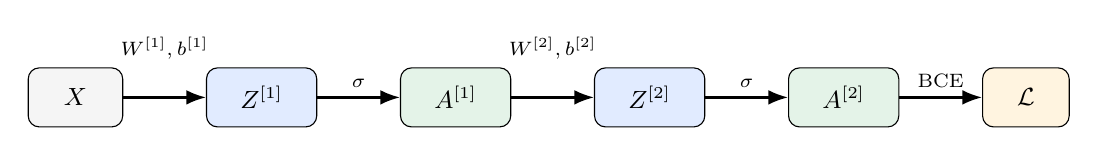
\begin{tikzpicture}[node distance=0.85cm and 1.05cm, every node/.style={font=\small}]
\node[draw,rounded corners,fill=SoftGray,minimum width=1.2cm,minimum height=0.75cm]
    (X)  {$X$};
\node[draw,rounded corners,fill=SoftBlue,right=of X,minimum width=1.4cm,minimum height=0.75cm]
    (Z1) {$Z^{[1]}$};
\node[draw,rounded corners,fill=SoftGreen,right=of Z1,minimum width=1.4cm,minimum height=0.75cm]
    (A1) {$A^{[1]}$};
\node[draw,rounded corners,fill=SoftBlue,right=of A1,minimum width=1.4cm,minimum height=0.75cm]
    (Z2) {$Z^{[2]}$};
\node[draw,rounded corners,fill=SoftGreen,right=of Z2,minimum width=1.4cm,minimum height=0.75cm]
    (A2) {$A^{[2]}$};
\node[draw,rounded corners,fill=SoftOrange,right=of A2,minimum width=1.1cm,minimum height=0.75cm]
    (L)  {$\mathcal{L}$};
\draw[-{Latex[length=2.5mm]},thick] (X)  -- node[above,yshift=10pt,font=\scriptsize]{$W^{[1]},b^{[1]}$} (Z1);
\draw[-{Latex[length=2.5mm]},thick] (Z1) -- node[above,font=\scriptsize]{$\sigma$}          (A1);
\draw[-{Latex[length=2.5mm]},thick] (A1) -- node[above,yshift=10pt,font=\scriptsize]{$W^{[2]},b^{[2]}$} (Z2);
\draw[-{Latex[length=2.5mm]},thick] (Z2) -- node[above,font=\scriptsize]{$\sigma$}          (A2);
\draw[-{Latex[length=2.5mm]},thick] (A2) -- node[above,font=\scriptsize]{BCE}               (L);
\end{tikzpicture}
\end{center}

\vspace{0.1cm}
The complete forward pass in matrix form:
\begin{align*}
Z^{[1]} &= W^{[1]} X + b^{[1]}, & A^{[1]} &= \sigma(Z^{[1]}), \\
Z^{[2]} &= W^{[2]} A^{[1]} + b^{[2]}, & A^{[2]} &= \sigma(Z^{[2]}), \\
\mathcal{L} &= -\tfrac{1}{m}\textstyle\sum\bigl[y\log A^{[2]} + (1-y)\log(1-A^{[2]})\bigr].
\end{align*}

\vspace{0.05cm}
\begin{block}{What backpropagation computes}
Starting from $\mathcal{L}$ and moving \textbf{right to left} along the graph, it applies the chain rule at each node to obtain $\partial\mathcal{L}/\partial W^{[2]}$, $\partial\mathcal{L}/\partial b^{[2]}$, $\partial\mathcal{L}/\partial W^{[1]}$, $\partial\mathcal{L}/\partial b^{[1]}$.
\end{block}
\end{frame}
%
%..................................................................
%
\begin{frame}{Applying the Chain Rule: Layer 2}
Referring to the forward-pass graph on the previous slide, for the \textbf{output layer} the chain rule gives:
\begin{align*}
&\frac{\partial \mathcal{L}}{\partial W^{[2]}} = \underbrace{\frac{\partial \mathcal{L}}{\partial A^{[2]}} \cdot \frac{\partial A^{[2]}}{\partial Z^{[2]}}}_{\textcolor{blue}{dZ2}} \cdot \frac{\partial Z^{[2]}}{\partial W^{[2]}}
\\[0.5em]
&\frac{\partial \mathcal{L}}{\partial b^{[2]}} = \textcolor{blue}{dZ2} \cdot \frac{\partial Z^{[2]}}{\partial b^{[2]}}
\end{align*}
\end{frame}
%
%..................................................................
%
\begin{frame}{Applying the Chain Rule: Layer 1}
For the \textbf{hidden layer}, the chain extends further back through the graph:
\begin{align*}
&\frac{\partial \mathcal{L}}{\partial W^{[1]}} = \underbrace{\textcolor{blue}{dZ2} \cdot \frac{\partial Z^{[2]}}{\partial A^{[1]}} \cdot \frac{\partial A^{[1]}}{\partial Z^{[1]}}}_{\textcolor{red}{dZ1}} \cdot \frac{\partial Z^{[1]}}{\partial W^{[1]}}
\\[0.5em]
&\frac{\partial \mathcal{L}}{\partial b^{[1]}} = \textcolor{red}{dZ1} \cdot \frac{\partial Z^{[1]}}{\partial b^{[1]}}
\end{align*}

\medskip
\textbf{Observe the recursive pattern:}
\begin{itemize}
\item Each layer computes a \textit{local error signal} $dZ^{[\ell]}$ from the layer above
\item The gradients for weights and biases follow the same form at every layer
\item This is the algorithm: \textbf{propagate $dZ$ backward, compute gradients locally}
\end{itemize}
\end{frame}
%
%..................................................................
%
\begin{frame}{Backpropagation Through Two Layers}
\framesubtitle{Complete Gradient Descent Update --- Putting It All Together}

\vspace{-0.15cm}

\begin{columns}[T]

% ---- LEFT: Gradient Formulas (Backpropagation) ----
\begin{column}{0.50\textwidth}

\small Step 1: \textbf{Compute Gradients (backward pass)}

{\small\color{layer2red}\textbf{Output Layer ($\ell = 2$):}}
{\small\color{layer2red}
\vspace{-0.15cm}
\begin{align*}
dZ^{[2]} &= A^{[2]} - y \\[-1pt]
dW^{[2]} &= \tfrac{1}{m}\, dZ^{[2]} \cdot {A^{[1]}}^{\!\top} \\[-1pt]
db^{[2]} &= \tfrac{1}{m} \textstyle\sum dZ^{[2]}
\end{align*}
}

{\small\color{layer1violet}\textbf{Hidden Layer ($\ell = 1$):}}
{\small\color{layer1violet}
\vspace{-0.15cm}
\begin{align*}
dZ^{[1]} &= {W^{[2]}}^{\!\top}\! \cdot dZ^{[2]} \odot A^{[1]}\!(1\!-\!A^{[1]}) \\[-1pt]
dW^{[1]} &= \tfrac{1}{m}\, dZ^{[1]} \cdot X^{\top} \\[-1pt]
db^{[1]} &= \tfrac{1}{m} \textstyle\sum dZ^{[1]}
\end{align*}
}

\end{column}

% ---- RIGHT: Update Rules (Gradient Descent) ----
\begin{column}{0.46\textwidth}

\small \textbf{Step 2: Update Parameters}

{\small\color{layer2red}\textbf{Output Layer ($\ell = 2$):}}
{\small
\begin{align*}
{\color{layer2red} \bm{W}^{[2]}} &\leftarrow W^{[2]} - {\color{updategreen}\eta} \cdot dW^{[2]} \\[3pt]
{\color{layer2red} \bm{b}^{[2]}} &\leftarrow b^{[2]} - {\color{updategreen}\eta} \cdot db^{[2]}
\end{align*}
}

{\small\color{layer1violet}\textbf{Hidden Layer ($\ell = 1$):}}
{\small
\begin{align*}
{\color{layer1violet} \bm{W}^{[1]}} &\leftarrow W^{[1]} - {\color{updategreen}\eta} \cdot dW^{[1]} \\[3pt]
{\color{layer1violet} \bm{b}^{[1]}} &\leftarrow b^{[1]} - {\color{updategreen}\eta} \cdot db^{[1]}
\end{align*}
}

\vspace{-0.15cm}

\colorbox{blue!8}{\parbox{0.92\linewidth}{\scriptsize
${\color{updategreen}\eta}$ = learning rate (hyperparameter)\\[1pt]
Repeat until convergence or early stopping.}}

\end{column}
\end{columns}

\end{frame}
%
%..................................................................
%
\begin{frame}{Backpropagation Through Two Layers}
\framesubtitle{Explicit Update Equations --- Fully Expanded Form}

\vspace{-0.1cm}

{\small Substituting the gradient expressions into $\theta \leftarrow \theta - \eta\, \nabla_\theta \mathcal{L}$\,:}

\vspace{0.15cm}

% ---- Layer 2 ----
{\small\color{layer2red}\textbf{Output Layer ($\ell = 2$):}}

\vspace{-0.05cm}

\begin{align}
{\color{layer2red}\bm{W}^{[2]}} &\leftarrow W^{[2]} \;-\; \frac{{\color{updategreen}\eta}}{m} \;\cdot\; \bigl(A^{[2]} - y\bigr) \;\cdot\; {A^{[1]}}^{\!\top} \label{eq:W2}\\[4pt]
{\color{layer2red}\bm{b}^{[2]}} &\leftarrow b^{[2]} \;-\; \frac{{\color{updategreen}\eta}}{m} \;\cdot\; \textstyle\sum \bigl(A^{[2]} - y\bigr) \label{eq:b2}
\end{align}

\vspace{0.05cm}

% ---- Layer 1 ----
{\small\color{layer1violet}\textbf{Hidden Layer ($\ell = 1$):}}

\vspace{-0.05cm}

\begin{align}
{\color{layer1violet}\bm{W}^{[1]}} &\leftarrow W^{[1]} \;-\; \frac{{\color{updategreen}\eta}}{m} \;\cdot\; \Bigl[\underbrace{{W^{[2]}}^{\!\top} \!\cdot\!\bigl(A^{[2]} - y\bigr)}_{\text{\scriptsize error backpropagated}} \;\odot\; \underbrace{A^{[1]}\!\bigl(1\!-\!A^{[1]}\bigr)}_{\text{\scriptsize local $\sigma'$}} \Bigr] \;\cdot\; X^{\top} \label{eq:W1}\\[4pt]
{\color{layer1violet}\bm{b}^{[1]}} &\leftarrow b^{[1]} \;-\; \frac{{\color{updategreen}\eta}}{m} \;\cdot\; \textstyle\sum \Bigl[{W^{[2]}}^{\!\top} \!\cdot\!\bigl(A^{[2]} - y\bigr) \;\odot\; A^{[1]}\!\bigl(1\!-\!A^{[1]}\bigr)\Bigr] \label{eq:b1}
\end{align}
\end{frame}
%______________________________________________________________________________
%
\subsection{Activation Functions Beyond the Sigmoid}
%______________________________________________________________________________
%
\begin{frame}{Why the Sigmoid Is Not Enough}

We have used the sigmoid $\sigma(z) = \frac{1}{1+e^{-z}}$ throughout.

\medskip
\textbf{Problems in deep networks:}
\begin{itemize}
    \item \textbf{Vanishing gradients:} $\sigma'(z) \leq 0.25$ always. In a network with $L$ layers, gradients shrink as $\sim (0.25)^L$.
    \item \textbf{Not zero-centered:} outputs are in $(0,1)$, causing zig-zag updates.
    \item \textbf{Saturation:} for large $|z|$, the gradient is nearly zero $\Rightarrow$ neurons stop learning.
\end{itemize}

\vspace{0.3cm}
\begin{alertblock}{Key insight}
Modern deep learning replaces the sigmoid with activation functions that do \textbf{not} suffer from these issues.
\end{alertblock}
\end{frame}
%
%..................................................................
%
\begin{frame}{The ReLU Activation}

The \textbf{Rectified Linear Unit} (Nair \& Hinton, 2010):
\[
g(z) = \max(z, 0)
\]

\begin{columns}
\begin{column}{0.48\textwidth}
\textbf{Advantages:}
\begin{itemize}
    \item Gradient is $1$ for $z>0$ $\Rightarrow$ no vanishing gradient
    \item Very fast to compute
    \item Induces \textbf{sparsity}: negative pre-activations are set to zero
    \item Empirically the most widely used activation
\end{itemize}
\end{column}
\begin{column}{0.48\textwidth}
\textbf{Derivative:}
\[
g'(z) = \begin{cases} 1 & z > 0 \\ 0 & z < 0 \end{cases}
\]
\textbf{Limitation:} ``dead neurons'' --- if $z < 0$ for all training inputs, the gradient is permanently zero.
\end{column}
\end{columns}

\end{frame}
%
%..................................................................
%
\begin{frame}{ReLU Variants}
\footnotesize
\begin{block}{Leaky ReLU (Maas et al., 2013)}
\[
g(z) = \begin{cases} z & z > 0 \\ \alpha z & z \leq 0 \end{cases}
\quad \text{with } \alpha \approx 0.01
\]
Prevents dead neurons by allowing a small gradient when $z < 0$.
\end{block}

\begin{block}{ELU --- Exponential Linear Unit (Clevert et al., 2015)}
\[
g(z) = \begin{cases} z & z > 0 \\ \alpha(e^z - 1) & z \leq 0 \end{cases}
\]
Smooth approximation that pushes mean activations closer to zero.
\end{block}

\begin{block}{Swish / SiLU (Ramachandran et al., 2017)}
\[
g(z) = z \cdot \sigma(z)
\]
Smooth, non-monotonic. Often outperforms ReLU in very deep networks.
\end{block}
\end{frame}
%
%..................................................................
%
\begin{frame}{Choosing an Activation Function --- Practical Guidelines}

\begin{center}
\renewcommand{\arraystretch}{1.4}
\begin{tabular}{l c c c}
\hline
\textbf{Activation} & \textbf{Range} & \textbf{Vanishing?} & \textbf{Typical use} \\
\hline
Sigmoid $\sigma(z)$ & $(0,1)$ & Yes & Output layer (binary) \\
Tanh & $(-1,1)$ & Yes & Recurrent networks \\
\textbf{ReLU} & $[0,\infty)$ & No & \textbf{Hidden layers (default)} \\
Leaky ReLU & $(-\infty,\infty)$ & No & Hidden layers \\
Softmax & $(0,1)^K$ & --- & Output (multiclass) \\
Linear & $(-\infty,\infty)$ & No & Output (regression) \\
\hline
\end{tabular}
\end{center}

\vspace{0.3cm}
\footnotesize
\textbf{Rule of thumb:}
\begin{itemize}
    \item \textbf{Hidden layers:} start with ReLU
    \item \textbf{Output layer:} match the problem (sigmoid for binary, softmax for multiclass, linear for regression)
\end{itemize}
\end{frame}
%__________________________________________________________________________
%
\section{Distributional Semantics and Dense Representations}
%__________________________________________________________________________
%
\begin{frame}{Why This Matters for NLP}
\begin{itemize}
    \item Neural networks are not introduced here to classify toy points forever.
    \item They matter because they allow us to \textbf{learn dense representations} of symbols, words, contexts, and documents.
    \item This is precisely the step that leads from classical vectorization to embeddings.
\end{itemize}

\vspace{0.2cm}
\begin{alertblock}{Transition}
Once we accept the idea that a model can learn an internal representation, the next question becomes: \emph{what kind of representation should language units have?}
\end{alertblock}
\end{frame}
%
%..................................................................
%
\begin{frame}{From Sparse Indicators to Dense Vectors}
\begin{columns}[T]
\begin{column}{0.49\textwidth}
\begin{block}{Sparse representation}
\begin{itemize}
    \item one-hot vectors,
    \item bag-of-words counts,
    \item TF--IDF features.
\end{itemize}
These are high-dimensional and mostly zero.
\end{block}
\end{column}
\begin{column}{0.49\textwidth}
\begin{block}{Dense representation}
\begin{itemize}
    \item few dimensions,
    \item continuous values,
    \item proximity meant to reflect similarity.
\end{itemize}
These are compact and learnable.
\end{block}
\end{column}
\end{columns}

\vspace{0.2cm}
\begin{alertblock}{Shift in perspective}
In sparse models, features are mostly specified by the analyst. In dense models, the representation itself is often learned from data.
\end{alertblock}
\end{frame}
%
%..................................................................
%
\begin{frame}{The Distributional Hypothesis}
\begin{block}{Core intuition}
\textbf{Words that occur in similar contexts tend to have similar meanings.}
\end{block}

\vspace{0.15cm}
\begin{itemize}
    \item This is the conceptual basis of \textbf{distributional semantics}.
    \item Meaning is not assumed to be given by a dictionary definition alone.
    \item Instead, meaning is inferred from patterns of co-occurrence and context.
\end{itemize}

\vspace{0.15cm}
\begin{exampleblock}{Example}
If the words \textit{bond}, \textit{yield}, \textit{coupon}, and \textit{maturity} frequently appear in related environments, a representation learner should place them near one another in a semantic space.
\end{exampleblock}
\end{frame}
%
%..................................................................
%
\begin{frame}{What Is an Embedding?}
\begin{itemize}
    \item An embedding maps a symbolic object into a vector in a continuous space.
    \item In NLP, the object may be a word, subword, sentence, document, or even an entire query.
    \item The main goal is to encode \textbf{similarity}, \textbf{structure}, and sometimes \textbf{task-relevant information} into geometry.
\end{itemize}

\vspace{0.2cm}
\begin{block}{For words}
A word embedding associates each token $w$ with a vector
\[
\vect{e}(w) \in \mathbb{R}^{d},
\]
where $d$ is much smaller than the vocabulary size.
\end{block}
\end{frame}
%
%..................................................................
%
\begin{frame}{Why Embeddings Are Attractive}
\begin{columns}[T]
\begin{column}{0.49\textwidth}
\begin{block}{Compared with one-hot vectors}
\begin{itemize}
    \item lower dimensionality,
    \item continuous geometry,
    \item similarity can be measured naturally,
    \item information can be shared across words.
\end{itemize}
\end{block}
\end{column}
\begin{column}{0.49\textwidth}
\begin{block}{Compared with count-based features}
\begin{itemize}
    \item better handling of lexical variation,
    \item more flexible use in neural models,
    \item easier composition into larger architectures.
\end{itemize}
\end{block}
\end{column}
\end{columns}

\vspace{0.2cm}
\begin{alertblock}{But note}
An embedding is not meaning itself. It is a learned \textbf{representation} that may capture useful regularities of meaning.
\end{alertblock}
\end{frame}
%
%..................................................................
%
\begin{frame}{A Geometric View of Meaning}
\begin{center}
\begin{tikzpicture}[scale=1.0]
\draw[->] (0,0) -- (5.1,0) node[right] {$e_1$};
\draw[->] (0,0) -- (0,4.4) node[above] {$e_2$};
\fill[Forest] (1.1,3.1) circle (2.6pt) node[above left] {bond};
\fill[Forest] (1.5,2.7) circle (2.6pt) node[below left] {yield};
\fill[Forest] (1.9,3.35) circle (2.6pt) node[above] {coupon};
\fill[DeepRed] (4.0,0.9) rectangle +(0.10,0.10) node[right] {river};
\fill[DeepRed] (4.25,1.25) rectangle +(0.10,0.10) node[right] {forest};
\fill[CourseBlue] (2.9,2.1) circle (2.6pt) node[right] {bank};
\draw[densely dotted] (1.1,3.1) -- (1.9,3.35);
\draw[densely dotted] (4.0,0.95) -- (4.3,1.3);
\end{tikzpicture}
\end{center}

\small
\textbf{Interpretation : } If training succeeds, words used in related contexts should occupy nearby regions of the vector space, while unrelated words should be farther apart.
\end{frame}
%
%..................................................................
%
\begin{frame}{Vector Arithmetic in Embedding Space}
 
One of the most discussed properties of Word2Vec embeddings is the emergence
of \textbf{linear relational structure}.
 
\medskip
 
The classic example:
\[
  \mathbf{e}(\text{king}) - \mathbf{e}(\text{man}) + \mathbf{e}(\text{woman})
  \;\approx\; \mathbf{e}(\text{queen}).
\]
 
\begin{center}
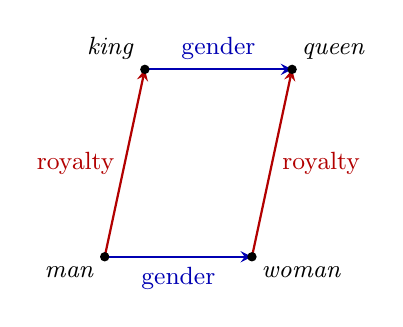
\begin{tikzpicture}[scale=0.85, >=stealth, every node/.style={font=\small}]
  % Points
  \coordinate (man) at (0,0);
  \coordinate (woman) at (2.2,0);
  \coordinate (king) at (0.6,2.8);
  \coordinate (queen) at (2.8,2.8);
 
  % Gender vectors
  \draw[->, thick, blue!70!black] (man) -- (woman)
    node[midway, below]{gender};
  \draw[->, thick, blue!70!black] (king) -- (queen)
    node[midway, above]{gender};
 
  % Royalty vectors
  \draw[->, thick, red!70!black] (man) -- (king)
    node[midway, left]{royalty};
  \draw[->, thick, red!70!black] (woman) -- (queen)
    node[midway, right]{royalty};
 
  % Labels
  \fill (man) circle (2pt) node[below left]{\textit{man}};
  \fill (woman) circle (2pt) node[below right]{\textit{woman}};
  \fill (king) circle (2pt) node[above left]{\textit{king}};
  \fill (queen) circle (2pt) node[above right]{\textit{queen}};
\end{tikzpicture}
\end{center}
 
\end{frame}
%
%..................................................................
%
\begin{frame}{Cosine Similarity Revisited}
If two embeddings are represented by vectors $\vect{u}$ and $\vect{v}$, a common similarity score is
\[
\cos(\theta) = \frac{\vect{u}^{\top}\vect{v}}{\|\vect{u}\|\,\|\vect{v}\|}.
\]

\vspace{0.2cm}
\begin{itemize}
    \item values close to $1$ indicate strong alignment,
    \item values close to $0$ indicate weak relation,
    \item values below $0$ indicate opposition in direction.
\end{itemize}

\vspace{0.2cm}
\begin{block}{Why cosine?}
It focuses on orientation rather than raw magnitude, which is often appropriate when we interpret vectors as semantic directions.
\end{block}
\end{frame}
%
%..................................................................
%
\begin{frame}{Static Word Embeddings}
The first widely successful generation of dense word embeddings was \textbf{static}:
\begin{itemize}
    \item one word,
    \item one vector,
    \item regardless of the sentence in which the word appears.
\end{itemize}

\vspace{0.2cm}
\begin{block}{Examples}
\begin{itemize}
    \item Word2Vec,
    \item GloVe,
    \item other pre-trained embedding collections.
\end{itemize}
\end{block}

\vspace{0.15cm}
\begin{alertblock}{Historical importance}
These models marked the transition from manually engineered lexical spaces to neural representation learning.
\end{alertblock}
\end{frame}
%__________________________________________________________________________
%
\section{Word2Vec: Learning Embeddings with a Shallow Neural Network}
%__________________________________________________________________________
%

\begin{frame}{What Is Word2Vec?}
Word2Vec is a method for learning word embeddings through a \textbf{shallow neural architecture}.
It transforms a symbolic word into a dense vector:
\[
w \;\mapsto\; e(w) \in \mathbb{R}^{k}, \qquad k \ll |V|,
\]
where $|V|$ is the vocabulary size.

\vspace{0.15cm}
\begin{block}{Why it was influential}
It made neural embedding learning computationally efficient and practically useful at scale --- and it showed that \textbf{meaningful geometry can emerge from a simple predictive task}.
\end{block}

\vspace{0.1cm}
\begin{alertblock}{Key question}
Where do the numbers in $e(w)$ come from, and why can a row of a weight matrix be interpreted as the representation of a word?
\end{alertblock}
\end{frame}
%
%..................................................................
%
\begin{frame}{The Training Principle: Context as a Proxy for Meaning}
	\begin{itemize}
		\item The input of word2vec is a text corpus and its output is a set of vectors known as feature vectors that represent words in that corpus. 
	\item The Word2Vec objective function causes the words that have a similar context to have similar embeddings. Thus in this vector space, these words are really close. 
		\item Word2vec is not a single algorithm but a combination of two techniques - CBOW(Continuous bag of words) and Skip-gram model.
		\item Both these techniques are shallow neural networks that learn weights which act as word vector representations. 
	\end{itemize}
\end{frame}
%
%..................................................................
%
\begin{frame}{The Training Principle: Context as a Proxy for Meaning}
	\begin{itemize}
		\item CBOW predicts the probability of a word to occur \textbf{given the words surrounding it}. We can consider a single word or a group of words. But for simplicity, we will take a single context word and try to predict a single target word.
		\item The English language contains almost 1.2 million words, making it impossible to include so many words in our example. So I will consider a small example in which we have only four words i.e. \textbf{live}, \textbf{home}, \textbf{they} and \textbf{at}. For simplicity, we will consider that the corpus contains only one sentence, that being, \textbf{They live at home}.
	\end{itemize}
\end{frame}
%
%..................................................................
%
\begin{frame}{Word2Vec : CBOW approach}
	First, we convert each word into a one-hot encoding form. Also, we will not consider all the words in the sentence but ll only take certain words that are in a window. 
	\begin{center}
	
\includegraphics[scale=0.6]{../05-pictures/chapter-02_pic_7.png}
	\end{center}
\end{frame}
%
%..................................................................
%
\begin{frame}{Word2Vec : CBOW approach}
	For example, for a window size equal to three, we only consider three words in a sentence. The middle word is to be predicted and the surrounding two words are fed into the neural network as context. The window is then slide and the process is repeated again.
	\begin{center}
	
\includegraphics[scale=0.6]{../05-pictures/chapter-02_pic_8.png}
	\end{center}
\end{frame}
%
%..................................................................
%
\begin{frame}{Word2Vec : Skip-Gram Model}
	\begin{itemize}
		\item The Skip-gram model tries to predict the source context words (surrounding words) given a target word (the centre word)
		\item The working is conceptually similar to the CBOW, there is just a difference in the architecture of its NN and in the way the weight matrix is generated:	 
	\end{itemize}
	\begin{center}
	
\includegraphics[scale=0.4]{../05-pictures/chapter-02_pic_9.png}
	\end{center}
\end{frame}
%
%..................................................................
%
\begin{frame}{The Architecture: Two Weight Matrices}
Both model have a minimal structure: $
x_w \;\xrightarrow{\;W\;}\; h \;\xrightarrow{\;W'\;}\; z
$

\vspace{0.1cm}
\begin{center}
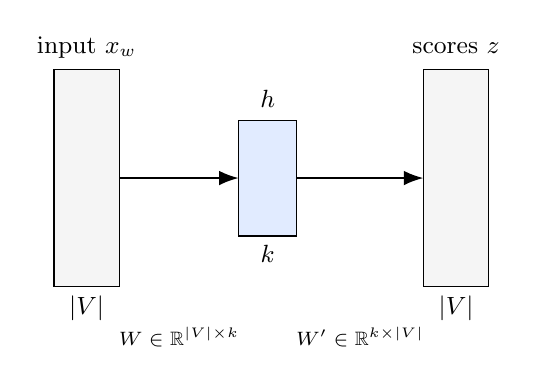
\begin{tikzpicture}[scale=0.92]
\draw[fill=SoftGray] (0,0) rectangle (0.9,3.0);
\draw[fill=SoftBlue] (2.55,0.7) rectangle (3.35,2.3);
\draw[fill=SoftGray] (5.1,0) rectangle (6.0,3.0);
\node[font=\small] at (0.45,3.3) {input $x_w$};
\node[font=\small] at (2.95,2.6) {$h$};
\node[font=\small] at (5.55,3.3) {scores $z$};
\draw[-{Latex[length=2.5mm]},thick] (0.9,1.5) -- (2.55,1.5)
      node[midway,below, yshift=-50pt,font=\scriptsize] {$W\in\mathbb{R}^{|V|\times k}$};
\draw[-{Latex[length=2.5mm]},thick] (3.35,1.5) -- (5.1,1.5)
      node[midway,below, yshift=-50,font=\scriptsize] {$W'\in\mathbb{R}^{k\times|V|}$};
\node[font=\small] at (0.45,-0.3) {$|V|$};
\node[font=\small] at (2.95,0.45) {$k$};
\node[font=\small] at (5.55,-0.3) {$|V|$};
\end{tikzpicture}
\end{center}

\begin{block}{The key structural fact}
$k \ll |V|$. The hidden layer is a \textbf{bottleneck}: it forces each word into a compact $k$-dimensional representation. The rows of $W$ are the embeddings.
\end{block}
\end{frame}
%
%..................................................................
%
\begin{frame}{The Architecture: Two Weight Matrices}
	\begin{center}
	
\includegraphics[scale=0.4]{../05-pictures/chapter-02_pic_10.png}
	\end{center}
\end{frame}
%
%..................................................................
%
\begin{frame}{Step 1: from a one-hot vector to the hidden layer}
The input word $w$ is represented by a one-hot vector:
\[
\bm{x}_w = (0,\dots,0,1,0,\dots,0)^\top \in \mathbb{R}^{V}.
\]

The hidden layer is computed as:
\[
\bm{h} = W^\top \bm{x}_w.
\]

\vspace{0.3cm}

Because $\bm{x}_w$ has a single entry equal to $1$, this multiplication simply selects the row of $W$ corresponding to word $w$.

\vspace{0.3cm}

Therefore:
\[
\bm{h} = \bm{v}_w.
\]

\vspace{0.3cm}

\textbf{Interpretation.} The hidden layer does not create a new arbitrary representation. It simply retrieves the embedding associated with the input word from the matrix $W$.
\end{frame}
%
%..................................................................
%
\begin{frame}{What does the hidden layer really do?}
Let the $i$-th row of $W$ be the vector associated with the $i$-th word in the vocabulary:
\[
W =
\begin{pmatrix}
--- \bm{v}_1^\top --- \\
--- \bm{v}_2^\top --- \\
\vdots \\
--- \bm{v}_V^\top ---
\end{pmatrix}.
\]

If word $w$ is the $j$-th word in the vocabulary, then $\bm{x}_w = \bm{e}_j$, where $\bm{e}_j$ is the $j$-th canonical basis vector. Hence:
\[
\bm{h} = W^\top \bm{e}_j = \bm{v}_j.
\]

\vspace{0.3cm}

So the hidden representation is nothing more than a \textbf{lookup operation} implemented as matrix multiplication. This is why the embedding matrix can be interpreted as a table storing one vector for each word.
\end{frame}
%
%..................................................................
%
\begin{frame}{Step 2: computing the output scores}
Once the hidden representation $\bm{h}$ has been obtained, the model computes a score for every candidate context word. The vector of pre-softmax scores is:
\[
\bm{u} = W'^\top \bm{h} \in \mathbb{R}^{V}.
\]

The score associated with a specific candidate context word $c$ is the $c$-th component of $\bm{u}$:
\[
u_c = {\bm{v}'_c}^\top \bm{h}.
\]

Since we already know that $\bm{h} = \bm{v}_w$, we obtain:
\[
u_c = {\bm{v}'_c}^\top \bm{v}_w.
\]

By definition the score is the \textbf{dot product} between:
\begin{itemize}
    \item the input embedding of the central word $w$,
    \item the output embedding of the candidate context word $c$.
\end{itemize}
\end{frame}
%
%..................................................................
%
\begin{frame}{Geometric interpretation}
Recall the identity:
\[
{\bm{v}'_c}^\top \bm{v}_w = \lVert \bm{v}'_c \rVert \, \lVert \bm{v}_w \rVert \cos \theta,
\]
where:
\begin{itemize}
    \item $\lVert \bm{v}'_c \rVert$ is the norm of the output embedding,
    \item $\lVert \bm{v}_w \rVert$ is the norm of the input embedding,
    \item $\theta$ is the angle between the two vectors.
\end{itemize}

\vspace{0.3cm}

Therefore the score is large when:
\begin{enumerate}
    \item the two vectors point in similar directions, that is, $\cos \theta$ is large,
    \item and/or the vectors have large norms.
\end{enumerate}

\textbf{Interpretation.} Word2vec learns a latent space in which word-context pairs that frequently co-occur tend to have vectors with a large dot product.
\end{frame}
%
%..................................................................
%
\begin{frame}{Step 3: from scores to probabilities}
The scores are transformed into conditional probabilities through the softmax:
\[
P(c \mid w) = \frac{\exp(u_c)}{\sum_{j=1}^{V} \exp(u_j)}.
\]

Substituting the expression for each score gives:
\[
P(c \mid w) = \frac{\exp\!\left({\bm{v}'_c}^\top \bm{v}_w\right)}{\sum_{j=1}^{V} \exp\!\left({\bm{v}'_j}^\top \bm{v}_w\right)}.
\]

Hence the probability assigned to a context word depends directly on the dot product between the two embeddings.

\textbf{Important consequence.} Increasing the dot product between $\bm{v}_w$ and $\bm{v}'_c$ increases the probability that the model assigns to observing $c$ in the context of $w$.
\end{frame}
%
%..................................................................
%
\begin{frame}{Why this interpretation is conceptually useful}
The dot product acts as a \textbf{compatibility score}.

\vspace{0.3cm}

If two words are statistically compatible in the training corpus, the optimization process pushes their corresponding vectors so that:
\[
{\bm{v}'_c}^\top \bm{v}_w
\]
becomes large.

\vspace{0.3cm}

This means that word2vec does not directly encode symbolic linguistic rules. Instead, it learns distributed vector representations in which:
\begin{itemize}
    \item similar contexts produce similar embeddings,
    \item useful semantic or syntactic regularities emerge from the geometry of the learned space,
    \item the score is a simple algebraic measure of how well one word predicts another.
\end{itemize}
\end{frame}
%
%..................................................................
%
\begin{frame}{A subtle but important point: two embedding spaces}
A common simplification is to speak about \textbf{the} embedding of a word. During training, however, word2vec maintains two different embeddings for each word:

\vspace{0.2cm}

\begin{center}
\begin{tabular}{lll}
\toprule
Representation & Symbol & Role \\
\midrule
Input embedding & $\bm{v}_w$ & used when the word is the center word \\
Output embedding & $\bm{v}'_w$ & used when the word is a context word \\
\bottomrule
\end{tabular}
\end{center}

So the score is more precisely:
\[
\text{score}(w,c) = {\bm{v}'_c}^\top \bm{v}_w.
\]

After training, one usually keeps:
\begin{itemize}
    \item only the input embeddings,
    \item or only the output embeddings,
    \item or some combination of both.
\end{itemize}
\end{frame}
%
%..................................................................
%
\begin{frame}{Matrix view of the whole mechanism}
The entire forward pass of the skip-gram model can be summarized compactly as:
\[
\bm{x}_w \in \mathbb{R}^{V}
\quad \longrightarrow \quad
\bm{h} = W^\top \bm{x}_w \in \mathbb{R}^{k}
\quad \longrightarrow \quad
\bm{u} = W'^\top \bm{h} \in \mathbb{R}^{V}.
\]

For a specific context word $c$:
\[
u_c = {\bm{v}'_c}^\top \bm{v}_w.
\]

\vspace{0.3cm}

Therefore the skip-gram architecture can be read as:
\begin{center}
\textbf{select the embedding of the input word} $\rightarrow$ \textbf{compare it with all output embeddings by dot products}.
\end{center}

\vspace{0.3cm}

This is the fundamental reason why the final score has a natural interpretation as a dot product between learned embedded representations.
\end{frame}
%
%..................................................................
%
\begin{frame}{Why Similar Words End Up Close}
When the corpus repeatedly contains pairs such as
\[
(\text{bank},\text{loan}),\quad(\text{bank},\text{interest})
\quad\text{and}\quad
(\text{lender},\text{loan}),\quad(\text{lender},\text{interest}),
\]
both \textit{bank} and \textit{lender} are trained against the \textbf{same context words}.

\vspace{0.15cm}
Their rows in $W$ therefore receive similar gradient updates, and over time:
\[
e_{\text{in}}(\text{bank}) \;\approx\; e_{\text{in}}(\text{lender}).
\]

\begin{block}{Distributional consequence}
Geometric proximity is not assumed. It \textbf{emerges} because similar prediction pressure produces similar parameter updates.
\end{block}
\end{frame}
%
%..................................................................
%
\begin{frame}{Why Similar Words End Up Close}
\begin{alertblock}{The pretext task and self-supervised learning}
Word2Vec is \textbf{not} a language model: nobody uses its predictions.
The prediction task is a \emph{pretext} --- its sole role is to generate the gradient signal that shapes $W$.
This is the first example in the course of \textbf{self-supervised learning}, a logic that reappears in BERT and GPT.
\end{alertblock}
\end{frame}
%__________________________________________________________________________
%
\section{GloVe and the Role of Global Co-occurrence}
%__________________________________________________________________________
%
\begin{frame}{Why Another Embedding Method?}
Word2Vec relies primarily on \textbf{local context windows}. This is powerful, but one may ask whether the representation should also exploit more explicitly the \textbf{global co-occurrence structure} of the corpus.

\vspace{0.2cm}
\begin{block}{GloVe idea}
GloVe, or \textbf{Global Vectors for Word Representation}, combines the embedding philosophy with global corpus statistics derived from word co-occurrence.
\end{block}
\end{frame}
%
%..................................................................
%
\begin{frame}{The Co-occurrence Matrix $X$}
  Count how often word $j$ appears in the context of word $i$
  (within a sliding window of, say, 10 words).

  \vspace{.5cm}
  \begin{columns}[T]
    \begin{column}{0.55\textwidth}
      \centering
      \small
      \begin{tabular}{l|ccccc}
        \toprule
        & \textbf{ice} & \textbf{steam} & \textbf{water} & \textbf{solid} & \textbf{gas} \\
        \midrule
        \textbf{ice}   & ---  & 12 & 58 & 47 & 8  \\
        \textbf{steam} & 12   & --- & 63 & 3  & 52 \\
        \textbf{water} & 58   & 63 & --- & 21 & 19 \\
        \textbf{solid} & 47   & 3  & 21 & --- & 1  \\
        \textbf{gas}   & 8    & 52 & 19 & 1  & --- \\
        \bottomrule
      \end{tabular}
    \end{column}
    \begin{column}{0.40\textwidth}
	\vspace{-.3cm}
      \begin{block}{Notation}
        $X_{ij}$\,: \# times $j$ appears near $i$\\[6pt]
        $X_i = \sum_{k} X_{ik}$\,: total context count\\[6pt]
        $P_{ij} = X_{ij}\,/\,X_i$\,: probability of $j$ given context~$i$
      \end{block}
    \end{column}
  \end{columns}

  \vspace{6pt}
  Think of it as a giant spreadsheet: rows are words, columns are words, and each cell records how often these two words appear near each other in the corpus.
\end{frame}
%
%..................................................................
%
\begin{frame}{GloVe's Key Insight: Ratios Reveal Meaning}
  Raw probabilities are noisy; \textbf{ratios} cancel out noise and isolate the semantic signal.

  \vspace{.5cm}
  \centering
  \normalsize
  \begin{tabular}{l c c c}
    \toprule
    \textbf{Probe word $k$}
      & $P(k\,|\,\text{ice})$
      & $P(k\,|\,\text{steam})$
      & $\bm{P_{\text{ice},k}\,/\,P_{\text{steam},k}}$ \\
    \midrule
    solid   & $1.9\times10^{-4}$ & $2.2\times10^{-5}$ & \textbf{8.9}\quad ($\gg 1$) \\
    gas     & $6.6\times10^{-5}$ & $7.8\times10^{-4}$ & \textbf{0.085}\quad ($\ll 1$) \\
    water   & $3.0\times10^{-3}$ & $2.2\times10^{-3}$ & \textbf{1.36}\quad ($\approx 1$) \\
    fashion & $1.7\times10^{-5}$ & $1.8\times10^{-5}$ & \textbf{0.96}\quad ($\approx 1$) \\
    \bottomrule
  \end{tabular}

  \vspace{.5cm}
  \begin{columns}[c]
    \begin{column}{0.30\textwidth}
      \centering
      {\Large $\gg 1$}\\[3pt]
      {\small $k$ relates more to \textbf{ice}}
    \end{column}
    \begin{column}{0.30\textwidth}
      \centering
      {\Large $\ll 1$}\\[3pt]
      {\small $k$ relates more to \textbf{steam}}
    \end{column}
    \begin{column}{0.30\textwidth}
      \centering
      {\Large $\approx 1$}\\[3pt]
      {\small $k$ is neutral to both}
    \end{column}
  \end{columns}
\end{frame}
%
%..................................................................
%
\begin{frame}{From Ratios to a Model --- Setup}
  The \textbf{ratio} $P_{ik}/P_{jk}$ carries a clean semantic signal.
  We want to learn \textbf{vectors} that capture it.

  \vspace{2pt}
  \begin{block}{Three kinds of vectors}
    \begin{itemize}
      \item $\vw_i \in \mathbb{R}^d$ --- the \textbf{target vector} for word $i$ (the word we are describing).
      \item $\vw_j \in \mathbb{R}^d$ --- the \textbf{target vector} for a second word $j$ (used for comparison with $i$).
      \item $\vwt_k \in \mathbb{R}^d$ --- the \textbf{context vector} for a probe word $k$ (the word we use to ``test'' the relationship). The tilde marks it as belonging to a \emph{separate} set of vectors.
    \end{itemize}
  \end{block}

  \vspace{1pt}
  \begin{block}{Recall: co-occurrence notation}
    $X_{ik}$\,: how many times $k$ appears near $i$.\;
    $X_i = \sum_k X_{ik}$\,: total context count.\;
    $P_{ik} = X_{ik}/X_i$\,: probability of $k$ given context~$i$.
  \end{block}

  \vspace{1pt}
  {\small\textit{Why two vector sets ($\vw$ and $\vwt$)?  A word plays two roles: sometimes it is the target, sometimes it is part of the surrounding context.}}
\end{frame}
%
%..................................................................
%
\begin{frame}{From Ratios to a Model --- Derivation}
  \textbf{Goal:} find $F$ such that
  $F(\vw_i,\, \vw_j,\, \vwt_k) = P_{ik}/P_{jk}$.

  \vspace{6pt}
  \textcolor{CourseBlue}{\textbf{Step 1}} --- \textbf{Use the \emph{difference} $\vw_i - \vw_j$, not both vectors separately.}\\[2pt]
  The ratio $P_{ik}/P_{jk}$ measures how $i$ and $j$ \emph{differ} w.r.t.\ the probe $k$, so $F$ should depend on $\vw_i - \vw_j$:
  \vspace{-4pt}
  \[ F\!\bigl(\vw_i - \vw_j,\;\; \vwt_k\bigr) \;=\; P_{ik}\,/\,P_{jk} \]

  \vspace{-6pt}
  \textcolor{CourseBlue}{\textbf{Step 2}} --- \textbf{Reduce two vectors to a scalar via a dot product.}\\[2pt]
  $F$ must output a \emph{number}, but $(\vw_i{-}\vw_j)$ and $\vwt_k$ are vectors.  The dot product is the simplest reduction:
  \vspace{-4pt}
  \[ F\!\bigl((\vw_i - \vw_j)^\top \vwt_k\bigr) \;=\; P_{ik}\,/\,P_{jk} \]

  \vspace{-6pt}
  \textcolor{CourseBlue}{\textbf{Step 3}} --- \textbf{Set $F = \exp$, so that subtraction becomes a ratio.}\\[2pt]
  Since $\exp(a-b) = e^a/e^b$, taking logs on both sides gives:
  \vspace{-4pt}
  \[ \vw_i^\top \vwt_k \;=\; \log P_{ik} \;=\; \log X_{ik} \;-\; \log X_i \]
\end{frame}
%
%..................................................................
%
\begin{frame}{Absorbing the Normalisation}
  The $\log X_i$ term in $\;\vw_i^\top \vwt_k = \log X_{ik} - \log X_i\;$ breaks the symmetry between $\vw$ and $\vwt$.

  \vspace{8pt}
  \textbf{Solution:} introduce \textbf{bias terms} $b_i$ and $\tilde{b}_j$ that absorb $\log X_i$ (and its symmetric counterpart):

  \vspace{6pt}
  \[
    \boxed{\;\vw_i^\top \vwt_j \;+\; b_i \;+\; \tilde{b}_j \;=\; \log X_{ij}\;}
  \]

  \vspace{6pt}
  This is the \textbf{core modelling equation} of GloVe:
  \begin{itemize}
    \item $\vw_i^\top \vwt_j$ captures the interaction between word $i$ and context word $j$.
    \item $b_i$ absorbs the ``popularity'' of word $i$ (how often it appears overall).
    \item $\tilde{b}_j$ absorbs the popularity of context word $j$.
  \end{itemize}

  \vspace{6pt}
  \begin{block}{Intuition}
    The biases act like \textbf{intercepts in a regression}: they soak up the overall frequency effects so that the dot product can focus purely on the \emph{relationship} between the two words.
  \end{block}
\end{frame}
%
%..................................................................
%
\begin{frame}{The GloVe Objective Function}
  \begin{block}{Loss function}
    \[
      J \;=\; \sum_{i,j=1}^{V} f(X_{ij})\;\bigl(\vw_i^\top \vwt_j + b_i + \tilde{b}_j - \log X_{ij}\bigr)^2
    \]
  \end{block}

  \vspace{6pt}
  \begin{columns}[T]
    \begin{column}{0.30\textwidth}
      \centering
      $\vw_i^\top\vwt_j + b_i + \tilde{b}_j$\\[6pt]
      {\small Model's prediction of $\log X_{ij}$}
    \end{column}
    \begin{column}{0.30\textwidth}
      \centering
      $\log X_{ij}$\\[6pt]
      {\small Observed target (log co-occurrence count)}
    \end{column}
    \begin{column}{0.30\textwidth}
      \centering
      $f(X_{ij})$\\[6pt]
      {\small Weighting function (controls each pair's influence)}
    \end{column}
  \end{columns}

  \vspace{10pt}
  Read it as: ``find vectors whose dot products match the log co-occurrence counts, weighting frequent pairs more.''
\end{frame}
%
%..................................................................
%
\begin{frame}{The Weighting Function $f(x)$}
  \begin{columns}[T]
    \begin{column}{0.52\textwidth}
      \vspace{6pt}
      \[
        f(x) = \begin{cases}
          (x\,/\,x_{\max})^\alpha & \text{if } x < x_{\max}\\[4pt]
          1 & \text{if } x \geq x_{\max}
        \end{cases}
      \]

      \vspace{8pt}
      \textbf{Why do we need this?}\\[4pt]
      Without weighting, ultra-common pairs like (``the'',~``of'') would dominate the loss and drown out the signal from rarer, more meaningful pairs.

      \vspace{6pt}
      The function $f$ acts as a \textbf{volume knob}: it turns down the influence of the most frequent pairs and gives rare pairs a fair chance.
    \end{column}
    \begin{column}{0.44\textwidth}
      \begin{block}{Design Properties}
        \begin{itemize}
          \item $f(0)=0$ --- skip zero-count pairs
          \item Non-decreasing --- frequent pairs still matter
          \item Saturates at $x_{\max}$ --- prevents ``the'' from dominating
          \item Typical: $\alpha=3/4$,\; $x_{\max}=100$
        \end{itemize}
      \end{block}

      \vspace{4pt}
      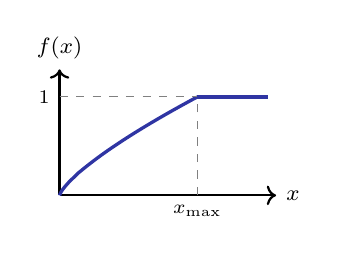
\begin{tikzpicture}[scale=0.5]
        \draw[->, thick] (0,0) -- (5.5,0) node[right] {\footnotesize $x$};
        \draw[->, thick] (0,0) -- (0,3.2) node[above] {\footnotesize $f(x)$};
        \draw[CourseBlue, very thick, domain=0:3.5, samples=100] plot (\x, {2.5*(\x/3.5)^0.75});
        \draw[CourseBlue, very thick] (3.5,2.5) -- (5.3,2.5);
        \draw[dashed, gray] (3.5,0) -- (3.5,2.5);
        \draw[dashed, gray] (0,2.5) -- (3.5,2.5);
        \node[below, font=\scriptsize] at (3.5,0) {$x_{\max}$};
        \node[left, font=\scriptsize] at (0,2.5) {$1$};
      \end{tikzpicture}
    \end{column}
  \end{columns}
\end{frame}
%
%..................................................................
%
\begin{frame}{Training GloVe in Practice}
  \begin{enumerate}
    \item \textbf{Build the co-occurrence matrix} ---
      Scan the entire corpus with a sliding window.
      Store all non-zero $X_{ij}$ entries (sparse matrix).

    \vspace{4pt}
    \item \textbf{Initialise vectors randomly} ---
      Two sets of vectors ($\vw$ and $\vwt$) plus biases $b_i$, $\tilde{b}_j$.
      Dimension $d$ is typically 50, 100, 200, or 300.

    \vspace{4pt}
    \item \textbf{Minimise $J$ with AdaGrad} ---
      Sample non-zero entries, compute gradients, update all parameters.
      AdaGrad adapts the learning rate per parameter --- important because word frequencies span many orders of magnitude.

    \vspace{4pt}
    \item \textbf{Combine the two vector sets} ---
      Final embedding $=$ $\vw_i + \vwt_i$.
      Averaging the two sets improves quality because the model treats them symmetrically.
  \end{enumerate}

  \vspace{4pt}
  Unlike Word2Vec, GloVe does \textbf{not} need multiple passes over raw text --- it only iterates over the (much smaller) set of \textbf{non-zero matrix entries}.
\end{frame}
%
%..................................................................
%
\begin{frame}{Key Hyperparameters}
  \centering
  \small
  \begin{tabular}{l l l}
    \toprule
    \textbf{Parameter} & \textbf{Typical} & \textbf{Effect} \\
    \midrule
    $d$ (dimension)    & 100--300   & Larger $\rightarrow$ richer, but more data needed \\
    Window size        & 5--15      & Larger $\rightarrow$ captures more topical similarity \\
    $x_{\max}$         & 100        & Cap on weighting function saturation \\
    $\alpha$           & 0.75       & Sub-linear scaling of co-occurrence counts \\
    Iterations         & 50--100    & More iterations $\rightarrow$ better convergence \\
    Learning rate      & 0.05       & AdaGrad handles per-parameter adaptation \\
    \bottomrule
  \end{tabular}

  \vspace{10pt}
  \begin{block}{Pre-trained vectors}
    The Stanford NLP Group provides pre-trained GloVe vectors on:
    \begin{itemize}
      \item Wikipedia 2014 + Gigaword 5 (6B tokens, 400K vocab)
      \item Common Crawl (42B and 840B tokens)
    \end{itemize}
    Available at: \url{https://nlp.stanford.edu/projects/glove/}
  \end{block}
\end{frame}
%
%..................................................................
%
\begin{frame}{Word Analogies: Linear Structure}
  GloVe vectors encode semantic relationships as \textbf{vector arithmetic}.

  \vspace{6pt}
  \begin{exampleblock}{Gender}
    \large\centering
    $\vec{\text{king}} - \vec{\text{man}} + \vec{\text{woman}} \;\approx\; \textbf{queen}$
  \end{exampleblock}
  \vspace{2pt}

  \begin{exampleblock}{Geography}
    \large\centering
    $\vec{\text{Paris}} - \vec{\text{France}} + \vec{\text{Italy}} \;\approx\; \textbf{Rome}$
  \end{exampleblock}
  \vspace{2pt}

  \begin{exampleblock}{Tense}
    \large\centering
    $\vec{\text{walking}} - \vec{\text{walked}} + \vec{\text{swam}} \;\approx\; \textbf{swimming}$
  \end{exampleblock}

  \vspace{4pt}
  This works because GloVe's log-bilinear structure naturally encodes differences as directions in vector space.
\end{frame}
%
%..................................................................
%
\begin{frame}{Benchmark Performance}
  \begin{block}{Word Analogy Task (semantic + syntactic)}
    \centering
    \small
    \begin{tabular}{l c c c}
      \toprule
      \textbf{Model} & \textbf{Dim} & \textbf{Corpus size} & \textbf{Accuracy (\%)} \\
      \midrule
      Word2Vec Skip-gram  & 300 & 1B   & 61.0 \\
      \textbf{GloVe}      & 300 & 6B   & \textbf{71.7} \\
      GloVe               & 300 & 42B  & \textbf{75.0} \\
      \bottomrule
    \end{tabular}

    \vspace{4pt}
    {\footnotesize Source: Pennington et al.\ (2014), Table~2}
  \end{block}

  \vspace{6pt}
  \begin{block}{Word Similarity Tasks (Spearman correlation)}
    GloVe achieves competitive or state-of-the-art results on WordSim-353, RG-65, MC-30, and other standard benchmarks, with performance scaling consistently with both corpus size and vector dimensionality.
  \end{block}

  \vspace{4pt}
  More data and more dimensions help, but with diminishing returns beyond $d \approx 300$.
\end{frame}
%
%..................................................................
%
\begin{frame}{GloVe vs.\ Word2Vec}
  \centering
  \small
  \begin{tabular}{l l l}
    \toprule
    & \textbf{GloVe} & \textbf{Word2Vec (Skip-gram)} \\
    \midrule
    \textbf{Approach}     & Count-based + regression    & Prediction-based (neural net) \\
    \textbf{Training data}& Co-occurrence matrix (pre-computed) & Raw text (online, window-by-window) \\
    \textbf{Statistics}   & Global (entire corpus at once) & Local (one window at a time) \\
    \textbf{Objective}    & Weighted least squares on log counts & Softmax / Negative sampling \\
    \textbf{Parallelism}  & Easy (matrix entries are independent) & Harder (sequential text) \\
    \textbf{Performance}  & Comparable; often wins on analogy & Comparable; often wins on similarity \\
    \bottomrule
  \end{tabular}

  \vspace{8pt}
  \begin{block}{A deeper connection}
    Levy \& Goldberg (2014) showed that Skip-gram with negative sampling \textbf{implicitly factorises a shifted PMI matrix} --- the two approaches are more similar than they appear.
  \end{block}
\end{frame}
%
%..................................................................
%
\begin{frame}{Applications in NLP and Finance}
  \begin{columns}[T]
    \begin{column}{0.47\textwidth}
      \begin{block}{Semantic Search}
        Find documents by \textbf{meaning}, not just keyword matching. Queries and documents live in the same vector space.
      \end{block}
      \vspace{4pt}
      \begin{block}{Sentiment Analysis}
        Pre-trained embeddings provide a strong initialisation for financial sentiment classifiers, even with limited labelled data.
      \end{block}
    \end{column}
    \begin{column}{0.47\textwidth}
      \begin{block}{Named Entity Recognition}
        Embeddings help detect company names, tickers, and financial entities in unstructured text (news, filings, reports).
      \end{block}
      \vspace{4pt}
      \begin{block}{Risk Factor Analysis}
        Cluster SEC filings by embedding similarity to discover emerging risk themes across industries and time periods.
      \end{block}
    \end{column}
  \end{columns}

  \vspace{6pt}
  In practice, GloVe embeddings are often used as the \textbf{initialisation layer} for downstream deep learning models (LSTMs, Transformers).
\end{frame}
%
%..................................................................
%
\begin{frame}{GloVe in the Embedding Landscape}
  \centering
  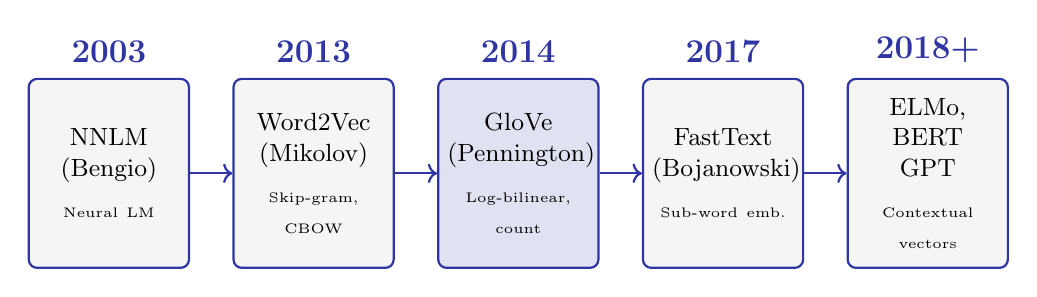
\begin{tikzpicture}[
    box/.style={
      rounded corners=3pt, draw=CourseBlue, thick,
      minimum width=2.0cm, minimum height=2.4cm,
      text width=1.8cm, align=center, font=\small
    },
    yearstyle/.style={font=\large\bfseries, text=CourseBlue}
  ]
    \node[box, fill=SoftGray] (b0) at (0, 0) {NNLM\\(Bengio)\\[4pt]{\tiny Neural LM}};
    \node[yearstyle, above=2pt] at (b0.north) {2003};

    \node[box, fill=SoftGray] (b1) at (2.6, 0) {Word2Vec\\(Mikolov)\\[4pt]{\tiny Skip-gram, CBOW}};
    \node[yearstyle, above=2pt] at (b1.north) {2013};

    \node[box, fill=CourseBlue!15] (b2) at (5.2, 0) {GloVe\\(Pennington)\\[4pt]{\tiny Log-bilinear, count}};
    \node[yearstyle, above=2pt] at (b2.north) {2014};

    \node[box, fill=SoftGray] (b3) at (7.8, 0) {FastText\\(Bojanowski)\\[4pt]{\tiny Sub-word emb.}};
    \node[yearstyle, above=2pt] at (b3.north) {2017};

    \node[box, fill=SoftGray] (b4) at (10.4, 0) {ELMo, BERT\\GPT\\[4pt]{\tiny Contextual vectors}};
    \node[yearstyle, above=2pt] at (b4.north) {2018+};

    \draw[->, thick, CourseBlue] (b0) -- (b1);
    \draw[->, thick, CourseBlue] (b1) -- (b2);
    \draw[->, thick, CourseBlue] (b2) -- (b3);
    \draw[->, thick, CourseBlue] (b3) -- (b4);
  \end{tikzpicture}

  \vspace{10pt}
  \begin{block}{Key takeaway}
    GloVe produces \textbf{static} embeddings (one vector per word regardless of context).
    Modern Transformers generate \textbf{contextual} embeddings, but GloVe remains valuable for its simplicity, interpretability, and efficiency.
  \end{block}
\end{frame}
%
%..................................................................
%
\begin{frame}{Glove: Key Takeaways}
  \begin{enumerate}
    \item Word embeddings turn words into \textbf{dense vectors} where geometry encodes meaning.

    \vspace{3pt}
    \item GloVe's key insight: \textbf{ratios of co-occurrence probabilities} distinguish relevant from irrelevant context words.

    \vspace{3pt}
    \item The objective is a \textbf{weighted least-squares regression} on log co-occurrence counts --- elegant and easy to optimise.

    \vspace{3pt}
    \item The weighting function $f$ prevents common words from dominating the loss.

    \vspace{3pt}
    \item GloVe vectors capture \textbf{linear relationships} (analogies) and transfer well to downstream tasks.

    \vspace{3pt}
    \item Though superseded by contextual models (BERT, GPT), GloVe remains a \textbf{clean, efficient, and interpretable} baseline.
  \end{enumerate}
\end{frame}
%__________________________________________________________________________
%
\section{Pre-Trained Embedding Models}
%__________________________________________________________________________
%
\begin{frame}{Pre-trained Embedding Models}
\begin{itemize}
    \item Training embeddings on a very large corpus can require substantial time and resources.
    \item For this reason, practitioners often use \textbf{pre-trained} Word2Vec or GloVe vectors.
    \item The idea is simple: representation learning is expensive, so we reuse embeddings learned from large generic corpora.
\end{itemize}

\vspace{0.2cm}
\begin{block}{Practical consequence}
Pre-trained embeddings made it possible to bring dense semantic information into downstream models even when the task-specific dataset was relatively small.
\end{block}
\end{frame}
%
%..................................................................
%
\begin{frame}{Embeddings in the Modeling Pipeline}
\begin{center}
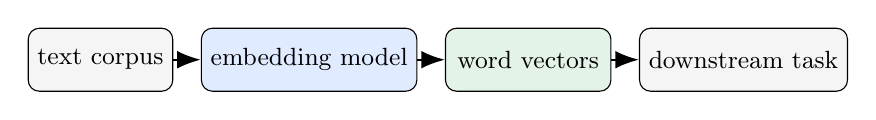
\begin{tikzpicture}[node distance=0.55cm and 0.35cm, every node/.style={font=\small}]
\node[draw, rounded corners, fill=SoftGray, minimum width=1.8cm, minimum height=0.8cm] (a) {text corpus};
\node[draw, rounded corners, fill=SoftBlue, right=of a, minimum width=2.0cm, minimum height=0.8cm] (b) {embedding model};
\node[draw, rounded corners, fill=SoftGreen, right=of b, minimum width=2.1cm, minimum height=0.8cm] (c) {word vectors};
\node[draw, rounded corners, fill=SoftGray, right=of c, minimum width=2.1cm, minimum height=0.8cm] (d) {downstream task};
\draw[-{Latex[length=3mm]}, thick] (a) -- (b);
\draw[-{Latex[length=3mm]}, thick] (b) -- (c);
\draw[-{Latex[length=3mm]}, thick] (c) -- (d);
\end{tikzpicture}
\end{center}

\vspace{0.2cm}
\begin{itemize}
    \item sentiment analysis,
    \item document classification,
    \item similarity,
    \item search,
    \item sequence labeling,
    \item many other downstream tasks.
\end{itemize}
\end{frame}
%__________________________________________________________________________
%
\section{Limits of Static Embeddings}
%__________________________________________________________________________
%
\begin{frame}{Domain Mismatch: Why General Embeddings May Mislead in Finance}
 
Pre-trained Word2Vec and GloVe vectors are typically trained on
Wikipedia or Google News.
 
\medskip
 
\begin{columns}[T]
\begin{column}{0.48\textwidth}
\begin{block}{General corpus}
\begin{itemize}
  \item \textit{bond} $\to$ near \textit{James Bond},
        \textit{movie}, \textit{spy}
  \item \textit{call} $\to$ near \textit{phone},
        \textit{dial}, \textit{ring}
  \item \textit{alpha} $\to$ near \textit{Greek},
        \textit{beta}, \textit{alphabet}
\end{itemize}
\end{block}
\end{column}
\begin{column}{0.48\textwidth}
\begin{block}{Financial corpus}
\begin{itemize}
  \item \textit{bond} $\to$ near \textit{yield},
        \textit{coupon}, \textit{maturity}
  \item \textit{call} $\to$ near \textit{option},
        \textit{strike}, \textit{put}
  \item \textit{alpha} $\to$ near \textit{excess return},
        \textit{benchmark}
\end{itemize}
\end{block}
\end{column}
\end{columns}
 
\bigskip
 
\begin{alertblock}{Implication for quantitative finance}
Using general-purpose embeddings on financial text can produce
semantically misleading similarities.  This motivates either
\textbf{domain-specific training} (embeddings on 10-K filings,
earnings calls, financial news) or \textbf{fine-tuning} ---
a theme we will revisit with contextual models like FinBERT in Lesson~3.
\end{alertblock}
 
\end{frame}
%
%..................................................................
%
\begin{frame}{The Main Limitation of Static Embeddings}
\begin{alertblock}{One word, one vector}
In Word2Vec and GloVe, each word type is assigned a single vector, no matter where the word appears.
\end{alertblock}

\vspace{0.15cm}
\begin{itemize}
    \item This is elegant and useful.
    \item But natural language is highly context-dependent.
    \item Many words are polysemous: they have multiple meanings.
\end{itemize}
\end{frame}
%
%..................................................................
%
\begin{frame}{Why Context Eventually Becomes Central}
Consider the word \textit{bank}:
\begin{itemize}
    \item in \emph{``the bank approved the loan''}, it refers to a financial institution;
    \item in \emph{``the fisherman sat on the bank''}, it refers to a river bank.
\end{itemize}

\vspace{0.2cm}
\begin{block}{Problem}
A static embedding gives both occurrences the same vector.
\end{block}

\vspace{0.15cm}
\begin{alertblock}{Implication}
If representation is to follow meaning more closely, the model must learn to modify a word's embedding according to its context.
\end{alertblock}
\end{frame}
%
%..................................................................
%
\begin{frame}{Another Example: \textit{current}}
\begin{columns}[T]
\begin{column}{0.48\textwidth}
\begin{block}{General representation}
A static embedding may place \textit{current} close to several semantic neighborhoods at once:
\begin{itemize}
    \item \textit{news}
    \item \textit{present}
    \item \textit{electricity}
\end{itemize}
\end{block}
\end{column}
\begin{column}{0.48\textwidth}
\begin{block}{Context-sensitive need}
In a sentence about circuits, the relevant relation should privilege the link between \textit{current} and \textit{electricity}, not the link between \textit{current} and \textit{news}.
\end{block}
\end{column}
\end{columns}

\vspace{0.2cm}
This is one of the conceptual pressures that eventually leads toward \textbf{contextual embeddings} and later toward \textbf{self-attention}.
\end{frame}
%
%..................................................................
%
\begin{frame}{A Historical Summary of the Transition}
\begin{center}
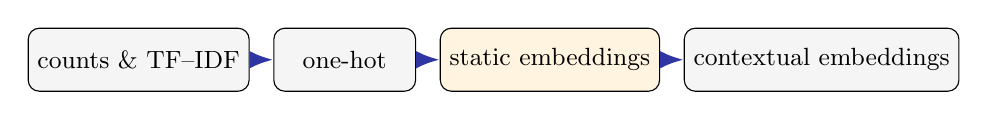
\begin{tikzpicture}[node distance=0.55cm and 0.3cm, every node/.style={font=\small}]
\node[draw, rounded corners, fill=SoftGray, minimum width=2.0cm, minimum height=0.8cm] (a) {counts \& TF--IDF};
\node[draw, rounded corners, fill=SoftGray, right=of a, minimum width=1.8cm, minimum height=0.8cm] (b) {one-hot};
\node[draw, rounded corners, fill=SoftOrange, right=of b, minimum width=2.2cm, minimum height=0.8cm] (c) {static embeddings};
\node[draw, rounded corners, fill=SoftGray, right=of c, minimum width=2.5cm, minimum height=0.8cm] (d) {contextual embeddings};
\draw[-{Latex[length=3mm]}, very thick, CourseBlue] (a) -- (b);
\draw[-{Latex[length=3mm]}, very thick, CourseBlue] (b) -- (c);
\draw[-{Latex[length=3mm]}, very thick, CourseBlue] (c) -- (d);
\end{tikzpicture}
\end{center}

\vspace{0.2cm}
\begin{block}{Interpretation}
Today's lesson has positioned us at the threshold of the transformer era: we now understand why distributed representations are necessary, why neural networks matter, and why static vectors are still not enough.
\end{block}
\end{frame}
%__________________________________________________________________________
%
\section{Conclusion and Bridge to Lesson 2b}
%__________________________________________________________________________
%
\begin{frame}{Conclusion: What We Have Built Today}
\begin{itemize}
    \item We introduced the idea of representation learning through neural models.
    \item We studied the logic of dense word embeddings, Word2Vec, and GloVe.
    \item We understood why static embeddings are powerful yet limited.
\end{itemize}

\vspace{0.2cm}
\begin{block}{Compact summary}
Lesson 1 asked how text can be represented at all. Lesson 2a asked how a model can \textbf{learn} such a representation. The next lesson will another fundamental property of language: sequentiality.
\end{block}
\end{frame}
%
%..................................................................
%
\begin{frame}{Main Takeaways}
\begin{enumerate}
    \item Neural networks matter in NLP not only as classifiers, but as \textbf{representation learners}.
    \item Word embeddings transform symbolic words into dense vectors whose geometry reflects contextual similarity.
    \item Word2Vec and GloVe are historically decisive because they made semantic geometry operational.
    \item Their main weakness is that they are \textbf{static}: one word still receives one vector.
\end{enumerate}
\end{frame}
%
%..................................................................
%
\begin{frame}{What We Have Built --- and What Is Still Missing}
\begin{columns}[T]
\begin{column}{0.48\textwidth}
\begin{block}{What Lesson 2a established}
\begin{itemize}
    \item Differentiable neurons enable gradient-based learning.
    \item Hidden layers learn \textbf{intermediate representations},
          not just classifiers.
    \item Word2Vec and GloVe show that \textbf{semantic geometry
          emerges} from predictive pressure on large corpora.
\end{itemize}
\end{block}
\end{column}
\begin{column}{0.48\textwidth}
\begin{alertblock}{What remains open}
\begin{itemize}
    \item Static embeddings assign \textbf{one vector per word},
          regardless of context.
    \item They treat the vocabulary as a set of independent symbols ---
          \textbf{no notion of order or sequence}.
    \item A model that reads language must process tokens
          \textbf{one after another}, accumulating meaning as it goes.
\end{itemize}
\end{alertblock}
\end{column}
\end{columns}

\vspace{0.2cm}
\begin{block}{The question for Lesson 2b}
How can a neural model process a sentence of \textbf{arbitrary length},
retain information from earlier tokens, and eventually produce an output
--- possibly of a \emph{different} length?
This requires a fundamentally new architectural idea: \textbf{recurrence}.
\end{block}
\end{frame}
%__________________________________________________________________________
%
\section{References}
%__________________________________________________________________________
%
\begin{frame}{References}
  \small
  \begin{thebibliography}{9}
    \bibitem{pennington2014}
      Pennington, J., Socher, R., \& Manning, C.\,D. (2014).
      GloVe: Global Vectors for Word Representation.
      \textit{Proc.\ EMNLP}, 1532--1543.

    \bibitem{mikolov2013}
      Mikolov, T., Sutskever, I., Chen, K., Corrado, G., \& Dean, J. (2013).
      Distributed Representations of Words and Phrases and their Compositionality.
      \textit{NeurIPS}.

    \bibitem{levy2014}
      Levy, O. \& Goldberg, Y. (2014).
      Neural Word Embedding as Implicit Matrix Factorization.
      \textit{NeurIPS}.

    \bibitem{bojanowski2017}
      Bojanowski, P., Grave, E., Joulin, A., \& Mikolov, T. (2017).
      Enriching Word Vectors with Subword Information.
      \textit{TACL}, 5, 135--146.

    \bibitem{devlin2019}
      Devlin, J., Chang, M.-W., Lee, K., \& Toutanova, K. (2019).
      BERT: Pre-training of Deep Bidirectional Transformers.
      \textit{NAACL-HLT}.
  \end{thebibliography}
\end{frame}
%
%===================================================================================================
%
\end{document}
%
%===================================================================================================
%
